\documentclass[11pt]{article}

\usepackage[a4paper, margin=2.8cm]{geometry}
\usepackage{amsmath, amssymb, amsthm}
\usepackage{booktabs}
\usepackage[normalem]{ulem}
\usepackage{float}
\usepackage{caption}
\usepackage[most]{tcolorbox}

% gray boxes with a subtle title strip, marking example material
\newtcolorbox{example}{
  breakable, enhanced,
  colback=gray!8, colframe=gray!50, boxrule=0.4pt, arc=1.5pt,
  colbacktitle=gray!22, coltitle=black!60,
  fonttitle=\small\scshape, title={example},
  toptitle=1.5pt, bottomtitle=1.5pt,
  left=7pt, right=7pt, top=5pt, bottom=5pt,
  before upper={\setlength{\parindent}{15pt}}}
\usepackage{graphicx}
\usepackage{colortbl}
\usepackage{tikz}

% lying probability bar, rightmost column of the truth tables;
% base scale: a full-width bar (1.3cm) is probability 1; the optional
% argument magnifies (used at 2x for the prior of Table 4)
\newcommand{\pbar}[2][1]{%
  \begin{tikzpicture}[baseline=-0.55ex]
    \useasboundingbox (0,-0.17) rectangle (1.3,0.17);
    \fill[blue!25] (0,-0.15) rectangle ({#2*1.3*#1},0.15);
  \end{tikzpicture}}

% subtle heat-map cell: darker blue for high values, lighter for low;
% shades are min-max normalized within their group (probabilities on
% [0,1]; the <s> and <dH(M)> rows jointly on [0.264, 1.104])
\newcommand{\hm}[1]{\cellcolor{blue!#1}}
\usepackage{pgfplots}
\pgfplotsset{compat=1.18}
\usetikzlibrary{svg.path}
\usetikzlibrary{tikzmark}
\usetikzlibrary{decorations.pathreplacing}

% forecast bar chart under the a\q matrices: one slot per question
% (width 2.1 = probability 1), one bar per answer with width M_{a,q}
% and height the branch drop in H(M) (y unit = 1 bit = 1.5cm); dashed
% line = the expected drop; fill = the question's <s> heatmap shade.
% \fslot{left x}{shade}{M_{0,q}}{drop a=0}{drop a=1}{<dH(M)>}
\newcommand{\fslot}[6]{%
  \draw[fill=blue!#2, draw=black!60, line width=0.3pt]
    (#1,0) rectangle ({#1+2.1*#3},#4);
  \draw[fill=blue!#2, draw=black!60, line width=0.3pt]
    ({#1+2.1*#3},0) rectangle ({#1+2.1},#5);
  \draw[dashed, black!70, line width=0.4pt] (#1,#6) -- ({#1+2.1},#6);
  \node[above, font=\scriptsize] at ({#1+1.05},{max(#4,#5)}) {$#6$};
  % answer digit at the bar base, or under the axis if the bar is tiny
  \pgfmathsetmacro{\yza}{ifthenelse(#4<0.2,-0.09,0.1)}
  \pgfmathsetmacro{\yzb}{ifthenelse(#5<0.2,-0.09,0.1)}
  \node[fill=white, inner sep=0.8pt, font=\tiny] at ({#1+1.05*#3},\yza) {$0$};
  \node[fill=white, inner sep=0.8pt, font=\tiny] at ({#1+1.05+1.05*#3},\yzb) {$1$};
}
% \fbrace{left x}{q label}: curly bracket + question label under a slot
\newcommand{\fbrace}[2]{%
  \draw[decorate, decoration={brace, mirror, amplitude=3pt}, black!70]
    (#1,-0.19) -- ({#1+2.1},-0.19);
  \node[below, font=\scriptsize] at ({#1+1.05},-0.28) {$\mathbf{#2}$};
}
% signed correlator bar chart, grouped by shell (groups 1-4-6-4-1);
% one entry per bar: x/value/mask/fill color; bars may go negative
\newcommand{\ledgerbars}[1]{%
\begin{center}
\begin{tikzpicture}[x=1cm, y=1cm]
  % alternating shell backdrops (spreadsheet banding), odd shells darker
  \fill[gray!10] (-0.35,-1.85) rectangle (0.40,1.3);
  \fill[gray!28] (0.40,-1.85) rectangle (2.85,1.3);
  \fill[gray!10] (2.85,-1.85) rectangle (6.40,1.3);
  \fill[gray!28] (6.40,-1.85) rectangle (8.85,1.3);
  \fill[gray!10] (8.85,-1.85) rectangle (9.60,1.3);
  \draw[->] (-0.6,-1.15) -- (-0.6,1.3);
  \foreach \y/\t in {-1/-1, 0/0, 1/+1}
    \draw (-0.66,\y) -- (-0.54,\y) node[left, font=\scriptsize] {$\t$};
  \draw[black!60, line width=0.4pt] (-0.6,0) -- (9.7,0);
  \foreach \x/\v/\l/\c in {#1} {
    \draw[fill=\c, draw=black!60, line width=0.3pt]
      ({\x-0.21},0) rectangle ({\x+0.21},\v);
    \node[rotate=90, anchor=east, font=\tiny] at (\x,-1.22) {\l};
  }
\end{tikzpicture}
\end{center}}

% \faxis: the shared y-axis and baseline of the forecast bar charts
\newcommand{\faxis}{%
  \draw[->] (-0.45,0) -- (-0.45,1.5);
  \node[above, font=\scriptsize] at (-0.45,1.5) {bits};
  \node[rotate=90, font=\scriptsize] at (-0.85,0.75) {$\Delta H(M)$};
  \foreach \y in {0,1}
    \draw (-0.51,\y) -- (-0.39,\y) node[left, font=\scriptsize] {$\y$};
  \draw[black!60, line width=0.4pt] (-0.45,0) -- (10.15,0);
}
\usepackage[colorlinks=true, linkcolor=blue!50!black, citecolor=blue!50!black, urlcolor=blue!50!black]{hyperref}

% the answer matrix M printed as a table: bold a-labels down the first
% column, bold q-labels along the first row, separated by rules
\newcommand{\Mtab}[4]{%
  \begin{array}{c|cc}
    \mathbf{a}\backslash\mathbf{q} & \mathbf{1} & \mathbf{0} \\
    \hline
    \mathbf{0} & #1 & #2 \\[2pt]
    \mathbf{1} & #3 & #4
  \end{array}}

% four-question version, for the n=2, m=1 guiding example
\newcommand{\MtabIV}[8]{%
  \begin{array}{c|cccc}
    \mathbf{a}\backslash\mathbf{q} & \mathbf{11} & \mathbf{10} & \mathbf{01} & \mathbf{00} \\
    \hline
    \mathbf{0} & #1 & #2 & #3 & #4 \\[2pt]
    \mathbf{1} & #5 & #6 & #7 & #8
  \end{array}}

\newtheorem{theorem}{Theorem}
\newtheorem{lemma}[theorem]{Lemma}
\newtheorem{definition}[theorem]{Definition}

\title{Leveraged Learning}
\author{Daniel Chernowitz}
\date{\today}

\begin{document}

\maketitle

This work rests on three insights. 
\begin{enumerate}
  \item Learning is the incremental ability to answer questions correctly that follow a pattern.
  \item The number of questions
reviewed is not the right measure of a learner's progress. What
counts is the information received from asking them. Not all
questions are created equal: about some, the learner already knows
a great deal a priori, and their answers count for less.
\item One can infer \emph{more} than a single bit from a yes--no
question, by exploiting the correlations of an intelligent prior:
an answer over here settles expectations over there. This ability
to extrapolate is codified here as \emph{leverage}.
\end{enumerate}


\section{A thought experiment}\label{sec:thought}

Let us start with a small thought experiment, by introducing
\emph{Werner the learner} (Figure~\ref{fig:werner}).

\begin{figure}[h]
\centering
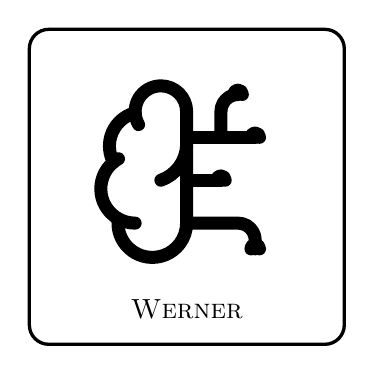
\begin{tikzpicture}[line cap=round, line join=round]
  % the box
  \draw[rounded corners=7pt, very thick] (-2.0,-2.05) rectangle (2.0,1.95);
  % Lucide brain-circuit icon (lucide.dev, ISC license), 24x24 viewBox;
  % svg.path coordinates are in pt (1 SVG unit = 1pt), hence the pt-based
  % scale and the y-flip for SVG's downward y-axis
  \begin{scope}[shift={(-1.31cm,1.45cm)}, xscale=3.1, yscale=-3.1,
                line width=4.7pt]
    \draw svg {M 12 5 a 3 3 0 1 0 -5.997 0.125 a 4 4 0 0 0 -2.526 5.77
               a 4 4 0 0 0 0.556 6.588 A 4 4 0 1 0 12 18 Z};
    \draw svg {M 9 13 a 4.5 4.5 0 0 0 3 -4};
    \draw svg {M 6.003 5.125 A 3 3 0 0 0 6.401 6.5};
    \draw svg {M 3.477 10.896 a 4 4 0 0 1 0.585 -0.396};
    \draw svg {M 6 18 a 4 4 0 0 1 -1.967 -0.516};
    \draw svg {M 12 13 h 4};
    \draw svg {M 12 18 h 6 a 2 2 0 0 1 2 2 v 1};
    \draw svg {M 12 8 h 8};
    \draw svg {M 16 8 V 5 a 2 2 0 0 1 2 -2};
    \draw svg {M 15.5 13 a 0.5 0.5 0 1 0 1 0 a 0.5 0.5 0 1 0 -1 0};
    \draw svg {M 17.5 3 a 0.5 0.5 0 1 0 1 0 a 0.5 0.5 0 1 0 -1 0};
    \draw svg {M 19.5 21 a 0.5 0.5 0 1 0 1 0 a 0.5 0.5 0 1 0 -1 0};
    \draw svg {M 19.5 8 a 0.5 0.5 0 1 0 1 0 a 0.5 0.5 0 1 0 -1 0};
  \end{scope}
  % name plate
  \node at (0,-1.6) {\textsc{Werner}};
\end{tikzpicture}
\caption{Werner the learner.}
\label{fig:werner}
\end{figure}

In this work, we model learning as the increased ability to give the
correct answer to questions, as more of the ground truth is revealed.
It is Werner's job to learn a pattern. The most basic shape of a
pattern is a \emph{binary map}, and the most basic binary map is a map
from one bit to one bit.

The cast of the experiment:
\begin{itemize}
  \item a \textbf{question} $q \in Q = \{0,1\}$;
  \item an \textbf{answer} $a \in A = \{0,1\}$;
  \item the \textbf{truth} $\psi: Q \to A$, the one fixed map nature
    uses to answer questions. $\psi$ is unknown to Werner. By definition then, $\psi(q) = a$.
\end{itemize}
There are exactly four candidate maps $\phi_j$ that $\psi$ could be
(Table~\ref{tab:fourmaps}): each of the two inputs can be sent to
either of the two outputs, independently. We index them by reading
the truth table $\phi_j(1)\,\phi_j(0)$ as a binary numeral: that
number \emph{is} $j$.

\begin{table}[H]
\centering
\begin{tabular}{c cc l}
\toprule
$j$ & $\phi_j(1)$ & $\phi_j(0)$ & name \\
\midrule
0 & 0 & 0 & constant $0$ \\
1 & 0 & 1 & NOT ($\lnot q$) \\
2 & 1 & 0 & identity ($q$) \\
3 & 1 & 1 & constant $1$ \\
\bottomrule
\end{tabular}
\caption{The four binary maps from one bit to one bit.}
\label{tab:fourmaps}
\end{table}

Now, if Werner is unintelligent, he has no preconceived notion of
which maps are more useful, more likely, or somehow more logical than
others. In practice, we would have to tell Werner the answer $a$ to every single question $q$,
before he has learned the whole pattern. 


We model this with a \textbf{uniform prior}: writing
$p_j = P(\psi = \phi_j)$ for Werner's belief, every candidate map
carries the same weight.

\begin{example}
For the four maps at hand:
\begin{equation}
  p_j = \tfrac{1}{4}, \qquad j = 0, 1, 2, 3.
\end{equation}
\end{example}

What does this belief predict? For each question $q$ separately, we
can tabulate the probability of each possible answer $a$: it is the
total belief in the maps that would answer $a$ to $q$,
\begin{equation}
  M_{a,q} \;=\; \sum_{j\,:\,\phi_j(q) = a} p_j .
\end{equation}
Arranged with one row per answer ($a = 0, 1$ from the top) and one
column per question ($q = 1, 0$ from the left, descending like the
digits of the numeral convention), these numbers form the matrix
$M$ - each column a probability distribution over answers, so $M$
is column-stochastic.

\begin{example}
Under the uniform prior, two of the four maps
answer $0$ and two answer $1$, at either question:
\begin{equation}
  M \;=\;
  \Mtab{M_{0,1}}{M_{0,0}}{M_{1,1}}{M_{1,0}}
  \;=\;
  \Mtab{p_0 + p_1}{p_0 + p_2}{p_2 + p_3}{p_1 + p_3}
  \;=\;
  \Mtab{\tfrac12}{\tfrac12}{\tfrac12}{\tfrac12}\;.
\end{equation}
Every column is a fair coin: the unintelligent Werner predicts
nothing about any answer before it is revealed.

Next, Werner gets to predict the answer to the question $q = 0$. By
his own belief it is a coin toss: $M_{0,0} = M_{1,0} = \tfrac12$.
Let us say the answer comes back $a = 1$. The \textbf{surprisal} of
this answer, to Werner, is $1$ bit, because the probability he
assigned to it was one half.
\end{example}

In general, when an event a belief holds
with probability $P$ actually occurs, its surprisal is
\begin{equation}
  s \;=\; -\log_2 P \quad \text{bits},
\end{equation}
here $s = -\log_2 M_{a,q}$ for answer $a$ arriving at question $q$.
Surprisal measures how much the received information deviates from
what was already expected: an answer held certain ($P = 1$) carries
$0$ bits --- nothing new; a coin toss carries exactly $1$ bit; and
the surprisal grows without bound as the answer gets more unexpected,
$P \to 0$. It is additive: the surprisal of two independent events
occurring is the sum of their surprisals, just as their probabilities
multiply.

Moreover, Werner can use a process of elimination --- an extreme form
of Bayes' rule --- to update his prior into a posterior. Semantically:
every candidate map that would have answered the question wrongly is
now \emph{ruled out}, not merely disfavored.

\begin{example}
The truth $\psi$ answered $1$ at $q = 0$, and a map with
$\phi_j(0) = 0$ cannot be $\psi$. This kills the constant-$0$ map
($j = 0$) and the identity ($j = 2$). The two survivors, NOT
($j = 1$) and constant $1$ ($j = 3$), both predicted the observed
answer, so this round of evidence does not distinguish between them
at all (Table~\ref{tab:elimination}).

\begin{center}
\begin{tabular}{c cc l}
\toprule
$j$ & $\phi_j(1)$ & $\phi_j(0)$ & name \\
\midrule
\tikzmark{strikeA}0 & 0 & $\mathbf{0}$ & constant $0$\tikzmark{strikeAend} \\
1 & 0 & 1 & NOT ($\lnot q$) \\
\tikzmark{strikeB}2 & 1 & $\mathbf{0}$ & identity ($q$)\tikzmark{strikeBend} \\
3 & 1 & 1 & constant $1$ \\
\bottomrule
\end{tabular}
% one continuous strike-through rule per eliminated row
\begin{tikzpicture}[overlay, remember picture]
  \draw[line width=0.5pt]
    ([shift={(-2pt,0.55ex)}]pic cs:strikeA) --
    ([shift={(2pt,0.55ex)}]pic cs:strikeAend);
  \draw[line width=0.5pt]
    ([shift={(-2pt,0.55ex)}]pic cs:strikeB) --
    ([shift={(2pt,0.55ex)}]pic cs:strikeBend);
\end{tikzpicture}
\captionof{table}{The candidate maps after the answer $\psi(0) = 1$:
the two maps with $\phi_j(0) = 0$ are ruled out.}
\label{tab:elimination}
\end{center}
\end{example}

The surviving ratio of believabilities must be preserved, and the
only update that does so is to renormalize the surviving weights to
sum to one. (This is Bayes' rule with a $0/1$ likelihood:
$P(\psi = \phi_j \mid a) \propto P(a \mid \phi_j)\, p_j$, and
$P(a \mid \phi_j)$ is $1$ for a map that answers $a$ and $0$ for a
map that does not.)

\begin{example}
The posterior is
\begin{equation}
  p' \;=\; \big(0,\ \tfrac12,\ 0,\ \tfrac12\big).
\end{equation}
Constructing the new answer matrix from $p'$ by the same recipe as
before:
\begin{equation}
  M' \;=\;
  \Mtab{p'_0 + p'_1}{p'_0 + p'_2}{p'_2 + p'_3}{p'_1 + p'_3}
  \;=\;
  \Mtab{\tfrac12}{0}{\tfrac12}{1}\;.
\end{equation}
So indeed, Werner knows the answer to $q = 0$ --- that column has
collapsed onto $a = 1$ --- and he is still as agnostic as possible
about the other answer: the $q = 1$ column remains a fair coin. He
gained $1$ bit of surprisal information, and cleaned up his table to
the tune of $1$ bit: the $q = 0$ column went from a full bit of
answer-uncertainty to none, while the $q = 1$ column is unchanged.

After the next question, $q = 1$, he learns $a = 1$ --- again a coin
toss beforehand ($M'_{1,1} = \tfrac12$), so again worth $1$ bit of
surprisal. Elimination now rules out NOT ($\phi_1(1) = 0$), leaving a
single survivor:
\begin{equation}
  p'' \;=\; \big(0,\ 0,\ 0,\ 1\big),
  \qquad
  M'' \;=\; \Mtab{0}{0}{1}{1}\;.
\end{equation}
So this is the constant map: $\psi = \phi_3$. Werner is done. Every
column is one-hot, and he will be able to answer all questions
correctly from now on.
\end{example}

\section{Intelligent priors}\label{sec:intelligent}

Now, let us assume that Werner knows \emph{something} about the world
before he starts.

\begin{example}
Let us say Werner knows the map is not constant. His belief then
spreads evenly over the two remaining candidates, NOT ($j = 1$) and
the identity ($j = 2$):
\begin{equation}
  p \;=\; \big(0,\ \tfrac12,\ \tfrac12,\ 0\big).
\end{equation}
Is he any better at predicting $\psi(0)$? Constructing $M$ by the
usual recipe:
\begin{equation}
  M \;=\;
  \Mtab{p_0 + p_1}{p_0 + p_2}{p_2 + p_3}{p_1 + p_3}
  \;=\;
  \Mtab{\tfrac12}{\tfrac12}{\tfrac12}{\tfrac12}\;.
\end{equation}
He is still just as bad as before: every column a fair coin.
\end{example}

So what has all this veteran wisdom about the nature of patterns in
the world bought him? His increased ability for \emph{inference}.

\begin{example}
Ask $q = 0$ again, and let the answer again come back $a = 1$ ---
again a coin toss beforehand, so again worth exactly $1$ bit of
surprisal. Elimination rules out the identity ($\phi_2(0) = 0$), and
the lone survivor is NOT:
\begin{equation}
  p' \;=\; \big(0,\ 1,\ 0,\ 0\big),
  \qquad
  M' \;=\; \Mtab{1}{0}{0}{1}\;.
\end{equation}
This time \emph{both} columns collapse at once. Werner received the
same single bit of surprisal as before, but cleaned up $2$ bits of
table: the answer at $q = 0$ he observed, and the answer at $q = 1$
he \emph{deduced}, without ever asking --- ruling out the constants
means $\phi(1) \neq \phi(0)$, so his prior held the two answers
perfectly anticorrelated, and settling one settles the other. He is
done after one question instead of two.
\end{example}

We say the information from the first answer was \textbf{leveraged}.
We will make this more precise in the upcoming sections.

\subsection{A one-parameter world}\label{sec:oneparam}

For more structure, let us relax the claim that there are \emph{no}
constant maps. Instead, we create a one-parameter world where the
prior probability that the map is constant is $p$, spread evenly
within each class (Table~\ref{tab:oneparam}):

\begin{table}[H]
\centering
\begin{tabular}{c cc l c}
\toprule
$j$ & $\phi_j(1)$ & $\phi_j(0)$ & name & $p_j$ \\
\midrule
0 & 0 & 0 & constant $0$ & $p/2$ \\
1 & 0 & 1 & NOT ($\lnot q$) & $(1-p)/2$ \\
2 & 1 & 0 & identity ($q$) & $(1-p)/2$ \\
3 & 1 & 1 & constant $1$ & $p/2$ \\
\bottomrule
\end{tabular}
\caption{The one-parameter prior: constant with probability $p$.}
\label{tab:oneparam}
\end{table}

\noindent
In vector form, and with the answer matrix constructed by the usual
recipe:
\begin{equation}
  \big(p_0,\ p_1,\ p_2,\ p_3\big)
  \;=\; \tfrac12\big(p,\ 1-p,\ 1-p,\ p\big),
  \qquad
  M \;=\; \Mtab{\tfrac12}{\tfrac12}{\tfrac12}{\tfrac12}\;,
\end{equation}
fair coins in every column, for every value of $p$.

How much is there to learn, in total? We account for the table as a
whole by declaring entropy \emph{extensive} over the columns --- the
answer-uncertainties of the columns simply add:
\begin{equation}\label{eq:HM}
  H(M) \;:=\; \sum_{q} H\big(M_{\cdot,q}\big),
  \qquad
  H\big(M_{\cdot,q}\big) \;:=\; -\sum_{a} M_{a,q}\,\log_2 M_{a,q}.
\end{equation}
Here both columns are fair coins carrying $1$ bit each, so the table
starts at its maximum: $H(M) = 2$ bits.

Now let us ask a question. Again we could use $q = 0$; by the
symmetry of the prior it actually does not matter for this argument.
And we are now going to talk about \emph{expected} values, instead
of realized ones: averages over the possible maps, denoted
$\langle\,\cdot\,\rangle$. Since we assume our prior is \emph{a
priori} correct --- nature draws the truth from the very distribution
Werner believes --- the average over $\psi$ simply zips with the
weights: $\langle X \rangle = \sum_j p_j\, X(\psi{=}\phi_j)$.

How much surprisal should Werner expect from asking a question $q$?
The answer comes back $a$ exactly when the truth answers $a$, which
under the zipped average happens with probability
$\sum_{j:\phi_j(q)=a} p_j = M_{a,q}$ --- the very probability Werner
assigned to it --- and when it does, it costs him $-\log_2 M_{a,q}$
of surprisal. Grouping the average over maps by the answer each map
gives:
\begin{equation}\label{eq:surprisal-entropy}
  \langle s_q \rangle
  \;=\; \sum_{j} p_j \,\big({-}\log_2 M_{\phi_j(q),\,q}\big)
  \;=\; \sum_{a} \underbrace{\sum_{j\,:\,\phi_j(q)=a} p_j}_{M_{a,q}}
        \big({-}\log_2 M_{a,q}\big)
  \;=\; \sum_{a} M_{a,q}\,\big({-}\log_2 M_{a,q}\big).
\end{equation}
The right-hand side is exactly the column entropy
$H(M_{\cdot,q})$ of equation~\eqref{eq:HM}: \textbf{the expected
surprisal of a question is the entropy of its column}. Each answer occurs with
exactly the probability Werner assigned to it, so his average
surprisal is his own uncertainty about that answer --- an identity
that will do a great deal of work in what follows.

For a two-answer column, this entropy is a function of a single
number, the probability $x$ of one of the two answers: the
\textbf{binary entropy function}
\begin{equation}\label{eq:binary-entropy}
  h(x) \;:=\; -x\log_2 x \;-\; (1-x)\log_2(1-x),
\end{equation}
zero at $x \in \{0, 1\}$ (a settled answer) and maximal, $1$ bit, at
the fair coin $x = \tfrac12$. For the first question here the column
is a fair coin, so
\begin{equation}
  \langle s_1 \rangle \;=\; H\big(M_{\cdot,0}\big)
  \;=\; h\big(\tfrac12\big) \;=\; 1 \text{ bit},
\end{equation}
whatever the value of $p$.

And the other column is now cleaned up. Breaking the update down over
the possible maps: with probability $\tfrac12$ the answer is $1$
(truth is NOT or constant $1$), with probability $\tfrac12$ it is $0$
(truth is FALSE or the identity), and
\begin{equation}
  M' \;=\;
  \underbrace{\Mtab{1-p}{0}{p}{1}}_{a_1 = 1,\ \text{prob } 1/2}
  \quad\text{or}\quad
  \underbrace{\Mtab{p}{1}{1-p}{0}}_{a_1 = 0,\ \text{prob } 1/2}\;.
\end{equation}
Either way, the asked column is one-hot and the unasked column is a
coin of bias $p$: what survives on $q = 1$ is precisely the
class uncertainty --- constant or not --- and nothing else. The total
entropy of the table is now
\begin{equation}
  H(M') \;=\; 0 + h(p) \;=\; h(p),
\end{equation}
a reduction of $2 - h(p)$ bits, purchased with a single bit of
surprisal. Define the \textbf{leverage after one question} as the
ratio of table entropy destroyed to surprisal received:
\begin{equation}
  L_1 \;:=\; \frac{2 - h(p)}{1} \;=\; 2 - h(p) \;\in\; [1, 2].
\end{equation}
The expected surprisal on the second question is, once more, the
entropy of its column,
\begin{equation}
  \langle s_2 \rangle \;=\; h(p) \;\leq\; 1 \text{ bit},
\end{equation}
after which the table is empty. Cumulatively over the two questions,
$1 + h(p)$ bits of received information reduced the table by the
full $2$ bits it started with, so the \textbf{cumulative leverage}
after two questions is
\begin{equation}
  L_2 \;:=\; \frac{2}{1 + h(p)} \;\in\; [1, 2].
\end{equation}
So our knowledge about the world has allowed us to be more certain
after our inference. Set
$p = \tfrac12$, and the prior is the uniform one of
Section~\ref{sec:thought}: $h = 1$, $L_1 = L_2 = 1$, and nothing is
leveraged at all. As $p$ skews further from $\tfrac12$, the
second question carries less and less expected information, and Werner's
potential for learning from it goes down with it. The column it could clean up is nearly settled already. In the limit $p = 0$, we recover the non-constant
world from the start of Section~\ref{sec:intelligent}. There is no
surprisal and no improvement to $M$ left in the second question at
all: it contributes nothing to denominator or enumerator, and $L_1 = L_2$. Figure~\ref{fig:oneparam} traces all three curves
between these extremes.

\begin{figure}[H]
\centering
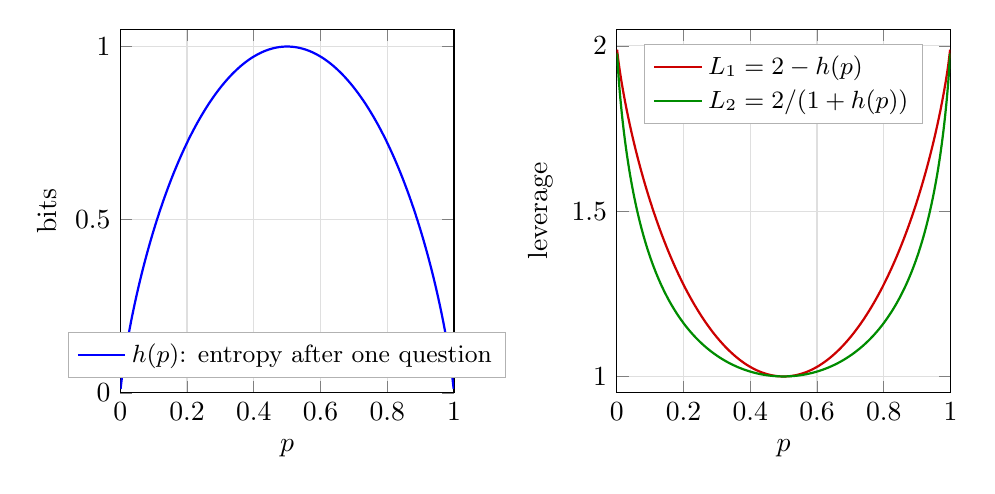
\begin{tikzpicture}[
  declare function={ hh(\x) = (-\x*ln(\x) - (1-\x)*ln(1-\x))/ln(2); }]
\begin{axis}[
  width=0.48\textwidth, height=6.2cm,
  xlabel={$p$},
  ylabel={bits},
  xmin=0, xmax=1, ymin=0, ymax=1.05,
  grid=major, grid style={gray!25},
  legend style={at={(0.5,0.04)}, anchor=south, draw=gray!60,
                fill=white, font=\small},
  legend cell align=left]
  \addplot[blue, thick, smooth, domain=0.001:0.999, samples=201]
    { hh(x) };
  \addlegendentry{$h(p)$: entropy after one question}
\end{axis}
\begin{axis}[
  xshift=0.52\textwidth,
  width=0.48\textwidth, height=6.2cm,
  xlabel={$p$},
  ylabel={leverage},
  xmin=0, xmax=1, ymin=0.95, ymax=2.05,
  grid=major, grid style={gray!25},
  legend style={at={(0.5,0.96)}, anchor=north, draw=gray!60,
                fill=white, font=\small},
  legend cell align=left]
  \addplot[red!80!black, thick, smooth, domain=0.001:0.999, samples=201]
    { 2 - hh(x) };
  \addlegendentry{$L_1 = 2 - h(p)$}
  \addplot[green!55!black, thick, smooth, domain=0.001:0.999, samples=201]
    { 2/(1 + hh(x)) };
  \addlegendentry{$L_2 = 2/(1+h(p))$}
\end{axis}
\end{tikzpicture}
\caption{The one-parameter world as a function of the constant-map
probability $p$. Left: the table entropy $h(p)$ remaining after one
question, in bits. Right: the one-question leverage $L_1$ and the
cumulative leverage $L_2$ after both questions. At $p = \tfrac12$
(the uniform prior) nothing is leveraged; toward the
deterministic-class extremes every answer doubles its value.}
\label{fig:oneparam}
\end{figure}

In general, in a larger world, if there are $d$ questions to disagree on between the two maps, the reader can convince themselves that the limit as $p \to 1$ is $L_1=d$. 

\section{The general case}\label{sec:general}

Now let us give the definitions in full generality. Questions are bit
strings of length $n$, and answers are bit strings of length $m$:
\begin{equation}
  q \in Q = \{0,1\}^n,
  \qquad
  a \in A = \{0,1\}^m,
\end{equation}
so there are $2^n$ distinct questions and $2^m$ possible answers to
each. As before, we read bit strings as the numbers they spell, using
the two interchangeably: $q \in \{0, \ldots, 2^n{-}1\}$ and
$a \in \{0, \ldots, 2^m{-}1\}$. The truth $\psi: Q \to A$ is one of
the candidate maps $\phi_j$; since each of the $2^n$ inputs can be
sent to any of the $2^m$ outputs independently, there are
\begin{equation}
  N \;=\; \big(2^m\big)^{2^n} \;=\; 2^{m\,2^n}
\end{equation}
of them, and the index $j$ is again the truth table read as a
numeral, now with $2^n$ digits in base $2^m$:
$j = \sum_q \phi_j(q)\,(2^m)^q$, running from the constant-$0$ map
($j = 0$) to the constant-$(2^m{-}1)$ map ($j = N{-}1$). Werner's
belief is a distribution over all of them, $\sum_{j=0}^{N-1} p_j = 1$.

\begin{example}
The example we will use to guide the general case is $n = 2$,
$m = 1$, which has $N = 2^{1 \cdot 4} = 16$ maps: every Boolean
function of the two input bits $b_1, b_0$, with $q = b_1 b_0$ read as
an ordinary binary number, $q = 2 b_1 + b_0$. Each $\phi_j$ in
Table~\ref{tab:sixteen} is shown as its truth table, printed in
descending question order $(11, 10, 01, 00)$ so that the answer to
question $q$ occupies the digit of weight $2^q$. The printed
string is exactly $j$ in binary (e.g.\ AND, which answers $1$ only to
$q = 11$, reads $1000$, so it is $j = 8$). The prior $p_j$ alongside
is conjured for illustration.

\begin{center}
\begin{tabular}{c |cccc| l c c}
\toprule
 & \multicolumn{4}{|c|}{$\phi_j(q)$} & & & \\
$j$ & $11$ & $10$ & $01$ & $00$ & name & $p_j$ & \\
\midrule
0  & 0 & 0 & 0 & 0 & FALSE (constant $0$) & 0.394 & \pbar[2]{0.394} \\
1  & 0 & 0 & 0 & 1 & $\lnot(b_1 \vee b_0)$ (NOR) & 0.010 & \pbar[2]{0.010} \\
2  & 0 & 0 & 1 & 0 & $\lnot b_1 \wedge b_0$ & 0.010 & \pbar[2]{0.010} \\
3  & 0 & 0 & 1 & 1 & $\lnot b_1$ & 0.010 & \pbar[2]{0.010} \\
4  & 0 & 1 & 0 & 0 & $b_1 \wedge \lnot b_0$ & 0.131 & \pbar[2]{0.131} \\
5  & 0 & 1 & 0 & 1 & $\lnot b_0$ & 0.010 & \pbar[2]{0.010} \\
6  & 0 & 1 & 1 & 0 & $b_1 \oplus b_0$ (XOR) & 0.010 & \pbar[2]{0.010} \\
7  & 0 & 1 & 1 & 1 & $\lnot(b_1 \wedge b_0)$ (NAND) & 0.010 & \pbar[2]{0.010} \\
8  & 1 & 0 & 0 & 0 & $b_1 \wedge b_0$ (AND) & 0.213 & \pbar[2]{0.213} \\
9  & 1 & 0 & 0 & 1 & $b_1 = b_0$ (XNOR) & 0.092 & \pbar[2]{0.092} \\
10 & 1 & 0 & 1 & 0 & $b_0$ (projection) & 0.040 & \pbar[2]{0.040} \\
11 & 1 & 0 & 1 & 1 & $b_1 \to b_0$ (IF THEN) & 0.010 & \pbar[2]{0.010} \\
12 & 1 & 1 & 0 & 0 & $b_1$ (projection) & 0.010 & \pbar[2]{0.010} \\
13 & 1 & 1 & 0 & 1 & $b_0 \to b_1$ (IF THEN) & 0.030 & \pbar[2]{0.030} \\
14 & 1 & 1 & 1 & 0 & $b_1 \vee b_0$ (OR) & 0.010 & \pbar[2]{0.010} \\
15 & 1 & 1 & 1 & 1 & TRUE (constant $1$) & 0.010 & \pbar[2]{0.010} \\
\bottomrule
\end{tabular}
\captionof{table}{The guiding example: all $16$ maps of the $n = 2$,
$m = 1$ hypothesis space, with a contrived prior
($\sum_j p_j = 1.000$).}
\label{tab:sixteen}
\end{center}
\end{example}

The answer matrix is defined by the same rule as before --- the total
belief in the maps that would answer $a$ to $q$:
\begin{equation}\label{eq:M-general}
  M_{a,q} \;=\; \sum_{j\,:\,\phi_j(q) = a} p_j,
\end{equation}
now a $2^m \times 2^n$ matrix, still with each column a probability
distribution over the possible answers: column-stochastic.

It is worth taking a moment to describe the constitution of this
matrix. Because of the enumeration of $j$ (the index \emph{is} the
truth table) the answer matrix has a natural structure: it is the
contraction of the belief vector $p$ with a fixed tensor with $\{0,1\}$ entries $E$,
summed along the map index,
\begin{equation}\label{eq:E}
  M_{a,q} \;=\; \sum_{j=0}^{N-1} E_{a,q,j}\; p_j,
  \qquad
  E_{a,q,j} \;:=\; \delta\big(\phi_j(q),\, a\big)
  \;=\; \delta\Big(\big\lfloor j \cdot 2^{-qm} \big\rfloor \bmod 2^m,\;
  a\Big).
\end{equation}
The second form is pure arithmetic on the index: by the
numeral convention, $\phi_j(q)$ is nothing but the $q$-th digit of
$j$ in base $2^m$, so $E$ never needs to be stored. Membership of
$j$ in the entry $M_{a,q}$ is read directly off the digits of $j$. This is a good thing, $E$ is astronomically large for even moderate $m$ and $n$.
For $m = 1$ this reduces to: bit $q$ of $j$ equals $a$. The tensor
$E$ is moreover sparse and perfectly regular: each question-slice ($q$ fixed)
holds exactly $N$ nonzero entries: every map answers exactly one
$a$ divided evenly over the $2^m$ answer rows, $N/2^m$ apiece.
Within a slice the nonzero row follows the odometer pattern of a
numeral system: runs of $(2^m)^q$ consecutive $j$ share a digit,
cycling through all $2^m$ rows with period $(2^m)^{q+1}$. 

The odometer pattern gives every entry of $M$ the same compact
closed form: for $m = 1$, bit $q$ of $j$ equals $0$ exactly when
$j \bmod 2^{q+1} < 2^q$, and equals $1$ otherwise.

\begin{example}
Each entry of $M$ collects the eight maps of Table~\ref{tab:sixteen}
whose truth table carries the right digit. Filling the entries in
--- note the period halving column by column, with the outer columns
written in their simplified forms, $j \bmod 16 < 8$ being simply
$j < 8$ and $j \bmod 2 < 1$ simply ``$j$ even'' --- and then
substituting the values of $p_j$:
\begin{equation}\label{eq:M16}
\begin{aligned}
  M \;&=\;
  \MtabIV{\scriptstyle\sum\limits_{j < 8} p_j}
         {\scriptstyle\sum\limits_{j \bmod 8 < 4} p_j}
         {\scriptstyle\sum\limits_{j \bmod 4 < 2} p_j}
         {\scriptstyle\sum\limits_{j\ \mathrm{even}} p_j}
         {\scriptstyle\sum\limits_{j \geq 8} p_j}
         {\scriptstyle\sum\limits_{j \bmod 8 \geq 4} p_j}
         {\scriptstyle\sum\limits_{j \bmod 4 \geq 2} p_j}
         {\scriptstyle\sum\limits_{j\ \mathrm{odd}} p_j}
  \\[10pt]
  &=\;
  \MtabIV{0.585}{0.779}{0.890}{0.818}
         {0.415}{0.221}{0.110}{0.182}\;.
\end{aligned}
\end{equation}
\end{example}

The update rule also carries over verbatim. When question $q$ is
asked and the answer $a = \psi(q)$ comes back, the process of
elimination reads, in one formula,
\begin{equation}\label{eq:update}
  p'_j \;=\; \frac{\delta\big(\phi_j(q),\, a\big)\; p_j}{M_{a,q}}
  \;=\; \frac{E_{a,q,j}\; p_j}{M_{a,q}}.
\end{equation}
The Kronecker delta performs the elimination. Only maps that agree with a survive and the division renormalizes the survivors,
whose total prior mass is exactly $M_{a,q}$ by
equation~\eqref{eq:M-general}. Note that one and the same number
prices the answer and funds the update: the event arrives with the
probability $M_{a,q}$, costs Werner $-\log_2 M_{a,q}$ bits of
surprisal, and its belief mass becomes the new unit of normalization. Every update shrinks the support by $2^{-m}$, radically thinning, especially for large $m$. The survivors live on a block-wave in $j$-space. The map determines the offset and frequency.
The total set of survivors depends on the set of asked questions, not the order: updating commutes. This is illustrated in the example below.

\begin{example}
Figure~\ref{fig:cull} makes the process visual for $n = m = 2$: a
schematic prior over $N = 4^4 = 256$ maps, drawn as vertical
lines with thickness representing weight. Each answer stops $3$ out of every $4$ surviving lines:
maps whose truth table carry a wrong digit at the asked question. Renormalization inflates the weight of the rest, so the total probability is always unit. Four questions cut
$256 \to 64 \to 16 \to 4 \to 1$, and the last line standing is the
truth. Note the regularity of the cull: each answer keeps a single
residue class of $j$, so the cadence of the survivors is regular.

\begin{center}
\resizebox{\linewidth}{!}{%
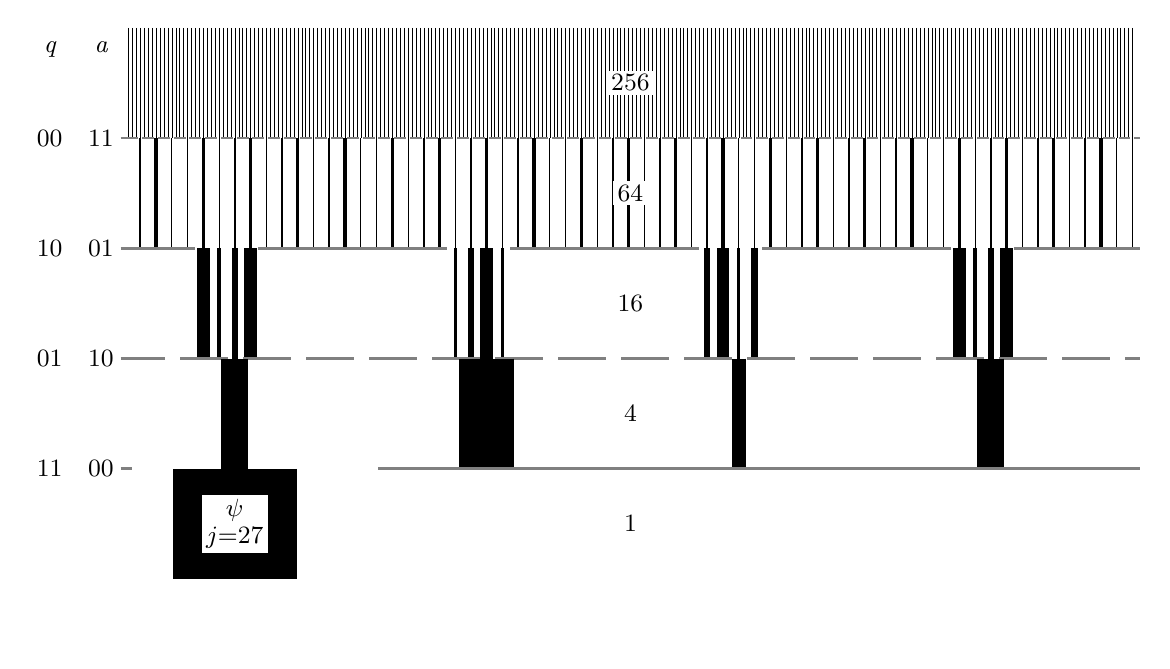
\begin{tikzpicture}[x=0.05cm, y=1cm]
  % label-column titles, tucked just below the starting line
  \node[anchor=north, font=\small\itshape] at (-20,-0.05) {q};
  \node[anchor=north, font=\small\itshape] at (-7,-0.05) {a};
  % round 0: all 256 maps
  \foreach \j in {0,...,255}
    \draw[line width=0.1pt] (\j,0) -- (\j,-1.4);
  % filter q=00, a=11: passes digit0 = 3, i.e. j mod 4 = 3
  \draw[gray, line width=1pt] (-2,-1.4) -- (2.5,-1.4);
  \foreach \k in {0,...,62}
    \draw[gray, line width=1pt] (4*\k+3.5,-1.4) -- (4*\k+6.5,-1.4);
  \draw[gray, line width=1pt] (255.5,-1.4) -- (257,-1.4);
  \node[font=\small] at (-20,-1.4) {$00$};
  \node[font=\small] at (-7,-1.4) {$11$};
  % survivors: j mod 4 = 3 (j = 4k+3), weight classes by k mod 3,
  % rotated so the eventual winner j=27 (k=6) carries the MIDDLE class:
  % k=0 -> 2, k=1 -> 4, k=2 -> 1; question order 00, 10, 01, 11;
  % layer masses 149 -> 39 -> 9 -> 2
  \foreach \j in {3,15,...,255}
    \draw[line width=0.6pt] (\j,-1.4) -- (\j,-2.8);
  \foreach \j in {7,19,...,247}
    \draw[line width=1.2pt] (\j,-1.4) -- (\j,-2.8);
  \foreach \j in {11,23,...,251}
    \draw[line width=0.3pt] (\j,-1.4) -- (\j,-2.8);
  % filter q=10, a=01: passes digit2 = 1, i.e. j mod 64 in [16,32);
  % windows nudged right so the finite-width survivor lines clear them
  \draw[gray, line width=1pt] (-2,-2.8) -- (17,-2.8);
  \foreach \s in {0,...,2}
    \draw[gray, line width=1pt] (64*\s+33,-2.8) -- (64*\s+81,-2.8);
  \draw[gray, line width=1pt] (225,-2.8) -- (257,-2.8);
  \node[font=\small] at (-20,-2.8) {$10$};
  \node[font=\small] at (-7,-2.8) {$01$};
  % survivors: digit 2 = 1, i.e. j mod 64 in {19,23,27,31},
  % all rescaled by 149/39
  \foreach \j in {23,83,95,155,215}
    \draw[line width=1.15pt] (\j,-2.8) -- (\j,-4.2);
  \foreach \j in {27,87,147,159,219}
    \draw[line width=2.29pt] (\j,-2.8) -- (\j,-4.2);
  \foreach \j in {19,31,91,151,211,223}
    \draw[line width=4.58pt] (\j,-2.8) -- (\j,-4.2);
  % filter q=01, a=10: passes digit1 = 2, i.e. j mod 16 in [8,12);
  % windows nudged right so the finite-width survivor lines clear them
  \draw[gray, line width=1pt] (-2,-4.2) -- (9.2,-4.2);
  \foreach \t in {0,...,14}
    \draw[gray, line width=1pt] (16*\t+13.2,-4.2) -- (16*\t+25.2,-4.2);
  \draw[gray, line width=1pt] (253.2,-4.2) -- (257,-4.2);
  \node[font=\small] at (-20,-4.2) {$01$};
  \node[font=\small] at (-7,-4.2) {$10$};
  % survivors: j mod 64 = 27, all rescaled by 39/9
  \draw[line width=9.93pt]  (27,-4.2)  -- (27,-5.6);
  \draw[line width=19.87pt] (91,-4.2)  -- (91,-5.6);
  \draw[line width=4.97pt]  (155,-4.2) -- (155,-5.6);
  \draw[line width=9.93pt]  (219,-4.2) -- (219,-5.6);
  % filter q=11, a=00: passes digit3 = 0, i.e. j mod 256 in [0,64);
  % the left stub is drawn a little longer than cell-exact, purely to
  % emphasize that the window's offset can be nonzero
  \draw[gray, line width=1pt] (-2,-5.6) -- (1,-5.6);
  \draw[gray, line width=1pt] (63.5,-5.6) -- (257,-5.6);
  \node[font=\small] at (-20,-5.6) {$11$};
  \node[font=\small] at (-7,-5.6) {$00$};
  % survivor: j = 27, rescaled by 9/2, labeled on a white patch
  \draw[line width=44.7pt] (27,-5.6) -- (27,-7.0);
  \node[fill=white, inner sep=1.5pt, font=\small, align=center]
    at (27,-6.3) {$\psi$\\[-1pt] $j{=}27$};
  % survivor counts per stage, superimposed mid-row on white patches
  \node[fill=white, inner sep=1.5pt, font=\small] at (127.5,-0.7) {$256$};
  \node[fill=white, inner sep=1.5pt, font=\small] at (127.5,-2.1) {$64$};
  \node[fill=white, inner sep=1.5pt, font=\small] at (127.5,-3.5) {$16$};
  \node[fill=white, inner sep=1.5pt, font=\small] at (127.5,-4.9) {$4$};
  \node[fill=white, inner sep=1.5pt, font=\small] at (127.5,-6.3) {$1$};
\end{tikzpicture}}
\captionsetup{skip=8pt}
\captionof{figure}{The update rule as a cull, for $n = m = 2$. All $256$
candidate maps start as vertical lines under a schematic prior. The truth is
the bitwise negation $\psi(q) = \lnot q$ ($j = 27$), and the four
questions are asked in the order $00, 10, 01, 11$. Each answer terminates the
$3/4$ of surviving maps whose truth-table digit at the asked question
disagrees. Every survivor's thickness, proportional to its
weight, is rescaled by the same renormalization factor, preserving
their ratios. After four questions a single map remains. Interestingly, the first cull's survivors are evenly spaced because it's the smallest question. After the three lowest $q$, even spacing returns.}
\label{fig:cull}
\end{center}
\end{example}

The total entropy of the table is extensive over the columns, exactly
as in equation~\eqref{eq:HM}:
\begin{equation}\label{eq:HM-general}
  H(M) \;=\; \sum_{q \in Q} H\big(M_{\cdot,q}\big)
  \;=\; -\sum_{q \in Q} \sum_{a \in A} M_{a,q} \log_2 M_{a,q}
  \;\;\leq\;\; m\,2^n,
\end{equation}
each column carrying at most $m$ bits (a uniform spread over its
$2^m$ answers). The ceiling $m\,2^n$ is the size of the entire truth
table in bits, and it is attained precisely by the uniform prior:
maximal ignorance prices every answer at full cost.

The belief itself carries an entropy as well, and we give its gap to
the table a name:
\begin{equation}\label{eq:C}
  H(p) \;=\; -\sum_{j=0}^{N-1} p_j \log_2 p_j,
  \qquad
  C \;:=\; H(M) - H(p) \;\geq\; 0.
\end{equation}
$H(p)$, Werner's uncertainty about the \emph{identity} of the truth,
obeys the same ceiling: a distribution over $N$ maps has entropy at
most $\log_2 N = m\,2^n$, attained again by the uniform prior.  The information in the
prior is not directly useful for prediction, but it is good to track. 

Why is $C>0$? The answers jointly determine the map, so $H(p)$ is the
\emph{joint} entropy of all $2^n$ answers, while $H(M)$ sums their
\emph{marginal} entropies and a joint entropy never exceeds the
sum of its marginals. Hence $H(p) \leq H(M)$, and the gap $C$, the
\textbf{total correlation} of the answers, is nonnegative: knowledge
stored in correlations \emph{between} answers, invisible to every
single column of $M$.

We choose this convention for $H(M)$ because in the ignorant case
\begin{enumerate}
  \item $H(M)$ is the total amount of information we must collect from questions to settle the map
  \item $H(M) = H(p)$, so the ignorance agrees in both bases, without correlations.
\end{enumerate}
Therefore, the scaling is sensible. How these quantities respond to an intelligent prior, is the main question of this work.

Let us watch these ledgers in motion by playing the guiding example
through all four questions. Werner can compute two forecasts for
every unasked question, in advance, from $M$ alone: the expected
surprisal $\langle s \rangle$, which by
equation~\eqref{eq:surprisal-entropy} is the entropy of that
question's column, and the expected drop
$\langle \Delta H(M) \rangle$ of the \emph{whole} table if that
question is asked next. This is the average over possible $a$, weighted by their probability (according to $M$):
\begin{equation}
  \langle s \rangle(q)
  \;=\; \sum_{a} M_{a,q}\,\big({-}\log_2 M_{a,q}\big),
\end{equation}
\begin{equation}
  \langle \Delta H(M) \rangle(q)
  \;=\; \sum_{a} M_{a,q}\,\Big[H(M) - H\big(M^{(q,a)}\big)\Big],
\end{equation}
where $M^{(q,a)}$ is the table after the update
rule~\eqref{eq:update} processes answer $a$ to question $q$. We know the column of $q$ will drop $\langle s \rangle(q)$ in entropy. But other columns will also respond.
The excess of the second over the first is
the expected transfer to unasked columns, and it can only be paid out
of correlations. We append both forecasts as extra rows under $M$.

\begin{example}

Werner plays greedily: always asking the question with the largest
forecast. The truth is AND ($\psi = \phi_8$).


\textbf{Question 1.} The starting state:
\[
  \begin{array}{c|cccc}
    \mathbf{a}\backslash\mathbf{q} & \mathbf{11} & \mathbf{10} & \mathbf{01} & \mathbf{00} \\
    \hline
    \mathbf{0} & \hm{20} 0.585 & \hm{27} 0.779 & \hm{31} 0.890 & \hm{29} 0.818 \\[2pt]
    \mathbf{1} & \hm{15} 0.415 & \hm{8} 0.221 & \hm{4} 0.110 & \hm{6} 0.182 \\
    \hline
    \langle s \rangle & \hm{30} 0.979 & \hm{21} 0.762 & \hm{10} 0.500 & \hm{18} 0.684 \\[2pt]
    \langle \Delta H(M) \rangle & \hm{35} 1.104 & \hm{22} 0.800 & \hm{12} 0.544 & \hm{22} 0.801
  \end{array}
\]
\begin{center}
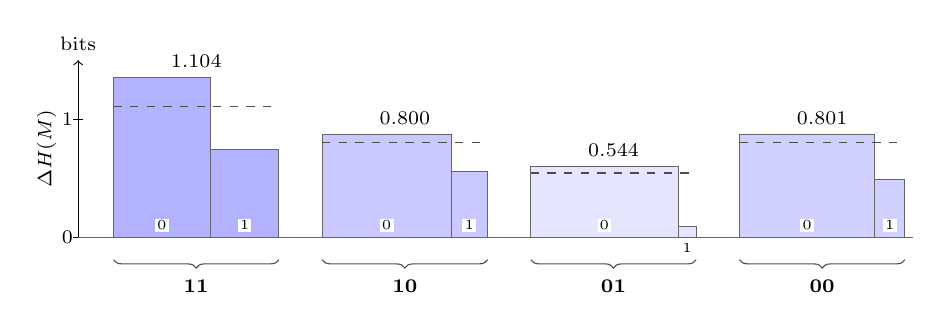
\begin{tikzpicture}[x=1cm, y=1.5cm]
  \faxis
  \fslot{0}{30}{0.585}{1.357}{0.748}{1.104}
  \fslot{2.65}{21}{0.779}{0.869}{0.556}{0.800}
  \fslot{5.30}{10}{0.890}{0.600}{0.088}{0.544}
  \fslot{7.95}{18}{0.818}{0.870}{0.491}{0.801}
  \fbrace{0}{11}\fbrace{2.65}{10}\fbrace{5.30}{01}\fbrace{7.95}{00}
\end{tikzpicture}
\end{center}
To see where the forecast entries come from, take $q = 11$: the
answer $a = 0$ arrives with probability $M_{0,11} = 0.585$ and would
drop $H(M)$ from $2.925$ to $1.569$; the answer $a = 1$ arrives with
probability $0.415$ and drops it only to $2.178$, so
\begin{align*}
  \langle s \rangle(11)
  &= 0.585\, (0.773) + 0.415\, (1.269) = 0.979, \\
  \langle \Delta H(M) \rangle(11)
  &= 0.585\, (1.357) + 0.415\, (0.748) = 1.104.
\end{align*}
Both forecast rows point to $q = 11$: it is the closest thing to a
coin on offer ($\langle s\rangle = 0.979$) and also moves the whole
table most, by a wide margin.
Werner asks it, and nature answers $a = 1$ (probability $0.415$,
surprisal $s_1 = 1.269$). Eight maps die:

\begin{center}
\begin{tabular}{c c l c c c}
\toprule
$j$ & $\phi_j(11)$ & name & $p_j$ & $p'_j$ & \\
\midrule
\tikzmark{w1a}0 & 0 & FALSE (constant $0$) & 0.394 & --- & \tikzmark{w1ae} \\
\tikzmark{w1b}1 & 0 & $\lnot(b_1 \vee b_0)$ (NOR) & 0.010 & --- & \tikzmark{w1be} \\
\tikzmark{w1c}2 & 0 & $\lnot b_1 \wedge b_0$ & 0.010 & --- & \tikzmark{w1ce} \\
\tikzmark{w1d}3 & 0 & $\lnot b_1$ & 0.010 & --- & \tikzmark{w1de} \\
\tikzmark{w1e}4 & 0 & $b_1 \wedge \lnot b_0$ & 0.131 & --- & \tikzmark{w1ee} \\
\tikzmark{w1f}5 & 0 & $\lnot b_0$ & 0.010 & --- & \tikzmark{w1fe} \\
\tikzmark{w1g}6 & 0 & $b_1 \oplus b_0$ (XOR) & 0.010 & --- & \tikzmark{w1ge} \\
\tikzmark{w1h}7 & 0 & $\lnot(b_1 \wedge b_0)$ (NAND) & 0.010 & --- & \tikzmark{w1he} \\
8 & 1 & $b_1 \wedge b_0$ (AND) & 0.213 & 0.513 & \pbar{0.513} \\
9 & 1 & $b_1 = b_0$ (XNOR) & 0.092 & 0.222 & \pbar{0.222} \\
10 & 1 & $b_0$ (projection) & 0.040 & 0.096 & \pbar{0.096} \\
11 & 1 & $b_1 \to b_0$ (IF THEN) & 0.010 & 0.024 & \pbar{0.024} \\
12 & 1 & $b_1$ (projection) & 0.010 & 0.024 & \pbar{0.024} \\
13 & 1 & $b_0 \to b_1$ (IF THEN) & 0.030 & 0.072 & \pbar{0.072} \\
14 & 1 & $b_1 \vee b_0$ (OR) & 0.010 & 0.024 & \pbar{0.024} \\
15 & 1 & TRUE (constant $1$) & 0.010 & 0.024 & \pbar{0.024} \\
\bottomrule
\end{tabular}
\begin{tikzpicture}[overlay, remember picture]
  \foreach \s/\e in {w1a/w1ae, w1b/w1be, w1c/w1ce, w1d/w1de,
                     w1e/w1ee, w1f/w1fe, w1g/w1ge, w1h/w1he}
    \draw[line width=0.5pt]
      ([shift={(-2pt,0.55ex)}]pic cs:\s) --
      ([shift={(2pt,0.55ex)}]pic cs:\e);
\end{tikzpicture}
\end{center}

The ledger:
\[
  H(M)\colon 2.925 \to 2.178, \qquad
  H(p)\colon 2.707 \to 2.093, \qquad
  C\colon 0.218 \to 0.085.
\]
Werner received $1.269$ bits but destroyed only $0.748$ bits of table.
Correlations point the right way only on average, not on every draw. In this case, Werner got the much less informative branch, and paid the premium price for it.
The destroyed-per-received ratio of this round is $0.589$: well below
$1$, anti-leverage.
\end{example}

Question 1 is a reminder that the forecast rows are
\emph{expectations}: they hold on average over many repetitions of
the experiment, and only if the world really does draw its truth $\psi$
from Werner's prior. On any single run the realized numbers are free
to deviate.

\begin{example}
\textbf{Question 2.} The state after the collapse, with fresh
forecasts:
\[
  \begin{array}{c|cccc}
    \mathbf{a}\backslash\mathbf{q} & \mathbf{11} & \mathbf{10} & \mathbf{01} & \mathbf{00} \\
    \hline
    \mathbf{0} & \hm{0} 0 & \hm{30} 0.855 & \hm{29} 0.831 & \hm{23} 0.658 \\[2pt]
    \mathbf{1} & \hm{35} 1 & \hm{5} 0.145 & \hm{6} 0.169 & \hm{12} 0.342 \\
    \hline
    \langle s \rangle & \text{---} & \hm{14} 0.596 & \hm{16} 0.655 & \hm{28} 0.927 \\[2pt]
    \langle \Delta H(M) \rangle & \text{---} & \hm{17} 0.670 & \hm{17} 0.677 & \hm{30} 0.983
  \end{array}
\]
\begin{center}
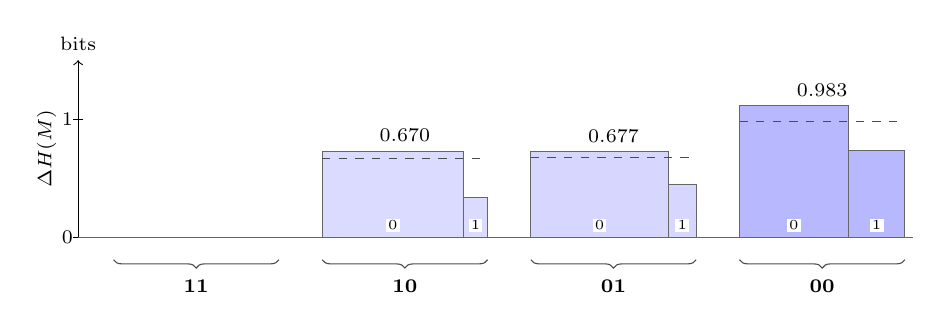
\begin{tikzpicture}[x=1cm, y=1.5cm]
  \faxis
  \fslot{2.65}{14}{0.855}{0.726}{0.341}{0.670}
  \fslot{5.30}{16}{0.831}{0.723}{0.451}{0.677}
  \fslot{7.95}{28}{0.658}{1.113}{0.733}{0.983}
  \fbrace{0}{11}\fbrace{2.65}{10}\fbrace{5.30}{01}\fbrace{7.95}{00}
\end{tikzpicture}
\end{center}
Greedy picks $q = 00$. Nature answers
$a = 0$ --- the answer Werner favored (probability $0.658$), so the
surprisal is only $s_2 = 0.604$ bits. Four of the eight die:

\begin{center}
\begin{tabular}{c c l c c c}
\toprule
$j$ & $\phi_j(00)$ & name & $p_j$ & $p'_j$ & \\
\midrule
8 & 0 & $b_1 \wedge b_0$ (AND) & 0.513 & 0.780 & \pbar{0.780} \\
\tikzmark{w2a}9 & 1 & $b_1 = b_0$ (XNOR) & 0.222 & --- & \tikzmark{w2ae} \\
10 & 0 & $b_0$ (projection) & 0.096 & 0.147 & \pbar{0.147} \\
\tikzmark{w2b}11 & 1 & $b_1 \to b_0$ (IF THEN) & 0.024 & --- & \tikzmark{w2be} \\
12 & 0 & $b_1$ (projection) & 0.024 & 0.037 & \pbar{0.037} \\
\tikzmark{w2c}13 & 1 & $b_0 \to b_1$ (IF THEN) & 0.072 & --- & \tikzmark{w2ce} \\
14 & 0 & $b_1 \vee b_0$ (OR) & 0.024 & 0.037 & \pbar{0.037} \\
\tikzmark{w2d}15 & 1 & TRUE (constant $1$) & 0.024 & --- & \tikzmark{w2de} \\
\bottomrule
\end{tabular}
\begin{tikzpicture}[overlay, remember picture]
  \foreach \s/\e in {w2a/w2ae, w2b/w2be, w2c/w2ce, w2d/w2de}
    \draw[line width=0.5pt]
      ([shift={(-2pt,0.55ex)}]pic cs:\s) --
      ([shift={(2pt,0.55ex)}]pic cs:\e);
\end{tikzpicture}
\end{center}

The ledger:
\[
  H(M)\colon 2.178 \to 1.065, \qquad
  H(p)\colon 2.093 \to 1.035, \qquad
  C\colon 0.085 \to 0.030.
\]
This time $1.113$ bits are destroyed for $0.604$ received. Where did
the extra $0.509$ come from? Partly from the favored answer arriving
--- the belief dropped $1.058$ against only $0.604$ paid --- and
partly from the store: $C$ fell by $0.055$.
Step ratio $1.842$. Cumulatively, however, $1.860$ destroyed per $1.873$
received gives a leverage of $0.993$ after 2 steps: still a hair
below $1$. Even a strong second round has not quite repaid the
expensive shock of question 1.
\end{example}

Why track $C$, when its step-by-step changes visibly do not match
the amounts deduced? Because on a single realized run the deduced
part has \emph{two} sources, and $C$ is the only quantity that
separates them. Writing $\Delta$ for the realized drops in one step,
\begin{equation}\label{eq:windfall-tower}
  \underbrace{\Delta H(M) - s}_{\text{deduced}}
  \;=\;
  \underbrace{\big[\Delta H(p) - s\big]}_{\text{windfall}}
  \;+\;
  \underbrace{\big[{-}\Delta C\big]}_{\text{tower}},
\end{equation}
an identity, since $H(M) = H(p) + C$ at every stage. The windfall is
luck: the realized surprisal undershooting (or overshooting) the
realized drop in belief entropy: zero in expectation. The tower
term is structure: a genuine withdrawal from the correlation store,
and the channel with a global guarantee. Over a complete run its
withdrawals sum to exactly the initial $C$, while the windfalls
average away. 

\begin{example}
\textbf{Question 3.} Two questions remain:
\[
  \begin{array}{c|cccc}
    \mathbf{a}\backslash\mathbf{q} & \mathbf{11} & \mathbf{10} & \mathbf{01} & \mathbf{00} \\
    \hline
    \mathbf{0} & \hm{0} 0 & \hm{32} 0.927 & \hm{29} 0.817 & \hm{35} 1 \\[2pt]
    \mathbf{1} & \hm{35} 1 & \hm{3} 0.073 & \hm{6} 0.183 & \hm{0} 0 \\
    \hline
    \langle s \rangle & \text{---} & \hm{5} 0.378 & \hm{18} 0.687 & \text{---} \\[2pt]
    \langle \Delta H(M) \rangle & \text{---} & \hm{6} 0.408 & \hm{19} 0.717 & \text{---}
  \end{array}
\]
\begin{center}
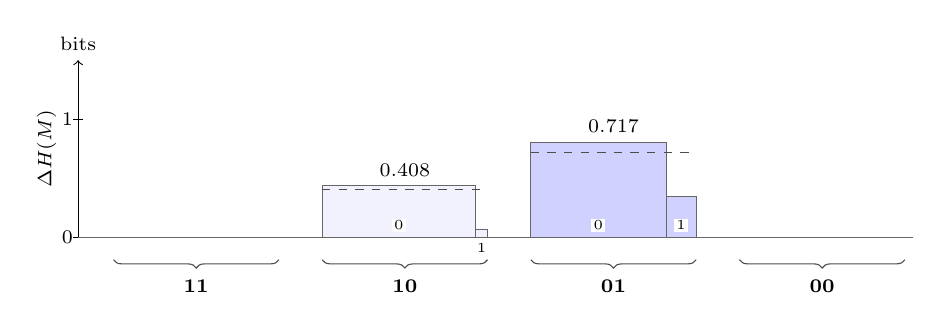
\begin{tikzpicture}[x=1cm, y=1.5cm]
  \faxis
  \fslot{2.65}{5}{0.927}{0.435}{0.065}{0.408}
  \fslot{5.30}{18}{0.817}{0.801}{0.343}{0.717}
  \fbrace{0}{11}\fbrace{2.65}{10}\fbrace{5.30}{01}\fbrace{7.95}{00}
\end{tikzpicture}
\end{center}
Greedy picks $q = 01$; nature answers $a = 0$ (probability $0.817$,
surprisal $s_3 = 0.292$). Two die:

\begin{center}
\begin{tabular}{c c l c c c}
\toprule
$j$ & $\phi_j(01)$ & name & $p_j$ & $p'_j$ & \\
\midrule
8 & 0 & $b_1 \wedge b_0$ (AND) & 0.780 & 0.955 & \pbar{0.955} \\
\tikzmark{w3a}10 & 1 & $b_0$ (projection) & 0.147 & --- & \tikzmark{w3ae} \\
12 & 0 & $b_1$ (projection) & 0.037 & 0.045 & \pbar{0.045} \\
\tikzmark{w3b}14 & 1 & $b_1 \vee b_0$ (OR) & 0.037 & --- & \tikzmark{w3be} \\
\bottomrule
\end{tabular}
\begin{tikzpicture}[overlay, remember picture]
  \foreach \s/\e in {w3a/w3ae, w3b/w3be}
    \draw[line width=0.5pt]
      ([shift={(-2pt,0.55ex)}]pic cs:\s) --
      ([shift={(2pt,0.55ex)}]pic cs:\e);
\end{tikzpicture}
\end{center}

The ledger:
\[
  H(M)\colon 1.065 \to 0.264, \qquad
  H(p)\colon 1.035 \to 0.264, \qquad
  C\colon 0.030 \to 0.
\]
Again a bargain: $0.801$ destroyed for a mere $0.292$ received, and the
cumulative ratio finally clears unity, at $1.229$. And note that $C$
has dropped to zero.
\end{example}

$C$ measures correlations that are not visible from $M$. If there's only one unknown column, there's nothing to infer. Put another way, usually, the binary maps are an overcomplete basis for $M$, because their number $N \gg \dim(M) = 2^{m+n}$.
That's not the case when the number of free parameters has been reduced by learning to 1 each.

\begin{example}
\textbf{Question 4.} One question, one heavily loaded coin:
\[
  \begin{array}{c|cccc}
    \mathbf{a}\backslash\mathbf{q} & \mathbf{11} & \mathbf{10} & \mathbf{01} & \mathbf{00} \\
    \hline
    \mathbf{0} & \hm{0} 0 & \hm{33} 0.955 & \hm{35} 1 & \hm{35} 1 \\[2pt]
    \mathbf{1} & \hm{35} 1 & \hm{2} 0.045 & \hm{0} 0 & \hm{0} 0 \\
    \hline
    \langle s \rangle & \text{---} & \hm{0} 0.264 & \text{---} & \text{---} \\[2pt]
    \langle \Delta H(M) \rangle & \text{---} & \hm{0} 0.264 & \text{---} & \text{---}
  \end{array}
\]
\begin{center}
\begin{tikzpicture}[x=1cm, y=1.5cm]
  \faxis
  \fslot{2.65}{0}{0.955}{0.264}{0.264}{0.264}
  \fbrace{0}{11}\fbrace{2.65}{10}\fbrace{5.30}{01}\fbrace{7.95}{00}
\end{tikzpicture}
\end{center}
The two forecasts now coincide: with $C = 0$ there is no transfer
left to hope for, and the last question can only be observed, not
leveraged. Nature answers $a = 0$ (probability $0.955$, surprisal
$s_4 = 0.066$):

\begin{center}
\begin{tabular}{c c l c c c}
\toprule
$j$ & $\phi_j(10)$ & name & $p_j$ & $p'_j$ & \\
\midrule
8 & 0 & $b_1 \wedge b_0$ (AND) & 0.955 & 1.000 & \pbar{1.000} \\
\tikzmark{w4a}12 & 1 & $b_1$ (projection) & 0.045 & --- & \tikzmark{w4ae} \\
\bottomrule
\end{tabular}
\begin{tikzpicture}[overlay, remember picture]
  \draw[line width=0.5pt]
    ([shift={(-2pt,0.55ex)}]pic cs:w4a) --
    ([shift={(2pt,0.55ex)}]pic cs:w4ae);
\end{tikzpicture}
\end{center}

The ledger closes:
\[
  H(M)\colon 0.264 \to 0, \qquad
  H(p)\colon 0.264 \to 0, \qquad
  C\colon 0 \to 0.
\]
The truth is AND. The step destroyed $0.264$ for $0.066$ received
(ratio $3.990$) --- not deduction this time, but luck: the destroyed
amount was fixed in advance (the column's full entropy), while the
realized surprisal undershot it because the likelier answer arrived.
In the split of equation~\eqref{eq:windfall-tower}: pure windfall,
tower $0$.

Cumulatively: $2.925$ bits of table
destroyed, all of it, for $2.231$ bits of
surprisal received: a run ratio of $1.311$. Most of the
realized $1.311$ was luck, not intelligence. Figure~\ref{fig:run21}
stacks the books after each question: what remains, plus what was
received. Once it dips below the starting entropy, our prior has done some work. 

\begin{center}
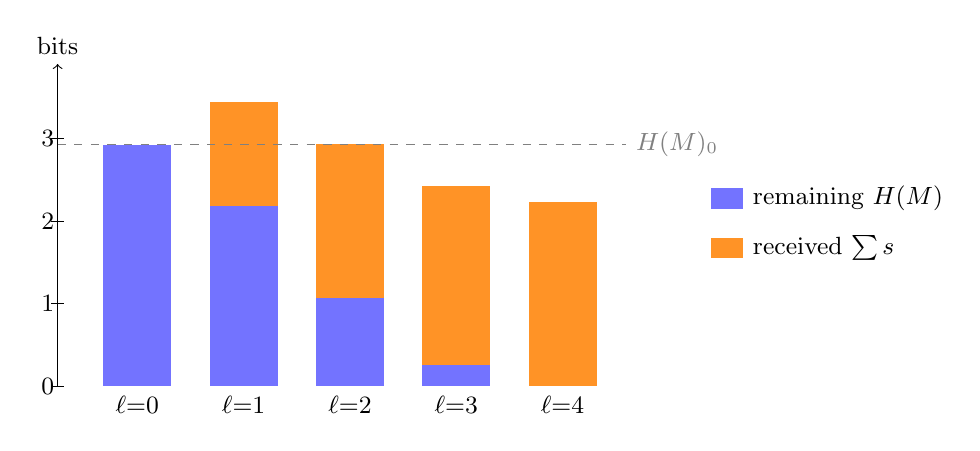
\begin{tikzpicture}[x=1.35cm, y=1.05cm]
  % axis
  \draw[->] (-0.75,0) -- (-0.75,3.9);
  \node[above, font=\small] at (-0.75,3.9) {bits};
  \foreach \y in {0,1,2,3}
    \draw (-0.81,\y) -- (-0.69,\y) node[left, font=\small] {$\y$};
  % l = 0
  \fill[blue!55] (-0.32,0) rectangle (0.32,2.925);
  % l = 1: stack tops at 3.446, well above H(M)_0
  \fill[blue!55] (0.68,0) rectangle (1.32,2.178);
  \fill[orange!85] (0.68,2.178) rectangle (1.32,3.446);
  % l = 2
  \fill[blue!55] (1.68,0) rectangle (2.32,1.065);
  \fill[orange!85] (1.68,1.065) rectangle (2.32,2.938);
  % l = 3
  \fill[blue!55] (2.68,0) rectangle (3.32,0.264);
  \fill[orange!85] (2.68,0.264) rectangle (3.32,2.429);
  % l = 4
  \fill[orange!85] (3.68,0) rectangle (4.32,2.231);
  % initial-total line
  \draw[dashed, gray] (-0.75,2.925) -- (4.6,2.925);
  \node[right, font=\small, gray] at (4.6,2.925) {$H(M)_0$};
  % x labels
  \foreach \l in {0,...,4}
    \node[below, font=\small] at (\l,0) {$\ell{=}\l$};
  % legend
  \fill[blue!55] (5.4,2.15) rectangle (5.7,2.4);
  \node[right, font=\small] at (5.7,2.27) {remaining $H(M)$};
  \fill[orange!85] (5.4,1.55) rectangle (5.7,1.8);
  \node[right, font=\small] at (5.7,1.67) {received $\sum s$};
\end{tikzpicture}
\captionof{figure}{The realized run through the guiding example:
remaining table entropy plus cumulative surprisal received, after
each question, against the initial total (dashed). The gap between
each stack and the line is the cumulative deduced part. At
$\ell = 1$ the stack tops out $0.521$ bits \emph{above} the
line --- the negative deduction of question 1, plainly visible. At
$\ell = 2$ the stack still grazes the line from above ($0.013$ bits);
only from $\ell = 3$ on do the stacks fall short of it, as genuine
deduction overtakes the early loss.}
\label{fig:run21}
\end{center}
\end{example}

If the prior is good, meaning it actual models reality (the prevalence of maps),
we expect graphs such as the one above to drop as questions come in.
The ratio of table entropy destroyed per bit of
surprisal received deserves a name.

The \textbf{leverage}. Run the protocol for $k$ rounds:
questions $q_1, \ldots, q_k$ are asked, the answers
$a_i = \psi(q_i)$ are each processed by the update
rule~\eqref{eq:update}, producing the tables $M^{(i)}$, and round $i$
costs the surprisal $s_i = -\log_2 M^{(i-1)}_{a_i,\,q_i}$. The
cumulative leverage after $k$ rounds is the table entropy destroyed
per bit of surprisal received:
\begin{equation}\label{eq:leverage}
  L_k \;:=\;
  \frac{H\big(M^{(0)}\big) - H\big(M^{(k)}\big)}
       {\sum_{i=1}^{k} s_i}\;.
\end{equation}
A leverage of $1$ is the uniform-prior baseline: every bit of table
entropy destroyed was paid for at face value, one bit of surprisal
each. Anything above $1$ is deduction --- table entropy removed
without ever being observed.

\section{Correlators}\label{sec:correlators}

What kind of operator is the update rule~\eqref{eq:update}? In map
space it is as simple as an operator gets: multiplication by a
diagonal $0/1$ mask, then renormalization. But there is a change of
basis in which the same operation becomes a \emph{convolution} with a
two-term kernel, and in which the correlation store $C$ stops being a
single number and becomes visible coordinate by coordinate. The main advantage is 
that the effect of each update is well tabulated beforehand into a small number of targeted parameters.

This
section builds that basis for $m = 1$; the final paragraph deals
with general $m$.

First, re-encode each answer as a spin,
\begin{equation}\label{eq:spin}
  \sigma_q(\phi_j) \;:=\; (-1)^{\phi_j(q)} \;\in\; \{+1, -1\},
\end{equation}
so answer $0 \mapsto +1$ and $1 \mapsto -1$. A pure relabeling, but
it buys the one algebraic fact everything below turns on:
$\sigma_q^2 = 1$.

The \textbf{Walsh--Hadamard transform} is built from a single
matrix. For one bit,
\begin{equation}\label{eq:hadamard}
  W \;=\; \begin{pmatrix} 1 & 1 \\ 1 & -1 \end{pmatrix},
  \qquad W_{c,b} \;=\; (-1)^{c\,b}, \quad c, b \in \{0,1\}.
\end{equation}
\begin{example}
Acting on a one-bit distribution,
\[
  W \binom{p_0}{p_1}
  \;=\; \binom{p_0 + p_1}{p_0 - p_1}
  \;=\; \binom{1}{\langle \sigma \rangle}:
\]
row $c = 0$ computes the normalization, row $c = 1$ the spin bias.
Distribution in, correlators out.
\end{example}

The normalization riding along is a redundancy. The original distribution also uses one variable more than its degrees of freedom.

\begin{example}
Tensoring two copies (the $n=1$ case) does the same for two bits at once:
\begin{equation}\label{eq:HH}
  W \otimes W \;=\;
  \begin{pmatrix}
    W & W \\
    W & -W
  \end{pmatrix}
  \;=\;
  \begin{pmatrix}
    1 & 1 & 1 & 1 \\
    1 & -1 & 1 & -1 \\
    1 & 1 & -1 & -1 \\
    1 & -1 & -1 & 1
  \end{pmatrix}
  \quad
  \begin{array}{l}
    \leftarrow c = 00\colon\ \text{sums to } 1 \\
    \leftarrow c = 01\colon\ \langle \sigma_0 \rangle \\
    \leftarrow c = 10\colon\ \langle \sigma_1 \rangle \\
    \leftarrow c = 11\colon\ \langle \sigma_1 \sigma_0 \rangle
  \end{array}
\end{equation}
\end{example}

The Kronecker product multiplies signs, so for any number $l$ of
tensor factors the entry at row $c$, column $j$ is
\begin{equation}\label{eq:kron}
  \big(W^{\otimes l}\big)_{c,j}
  \;=\; \prod_{b=0}^{l-1} (-1)^{c_b\, j_b}
  \;=\; (-1)^{\sum_b c_b\, j_b},
\end{equation}
with $c_b$, $j_b$ the $b$-th bits of the row and column indices;
every further tensor factor appends one more bit.

For $m = 1$ a map \emph{is} its truth table of $2^n$ bits --- the
numeral $j$ --- so Werner's belief is a vector of length
$N = 2^{2^n}$, and one transform computes every correlator at once:
\begin{equation}\label{eq:wht}
  \chi \;=\; W^{\otimes 2^n} p,
  \qquad
  \chi_S \;=\; \Big\langle \prod_{q \in S} \sigma_q \Big\rangle
  \;=\; \sum_{j=0}^{N-1} (-1)^{\sum_{q \in S} \phi_j(q)}\, p_j.
\end{equation}
Each row computes the \textbf{correlator} of one subset
$S \subseteq Q$ of questions. In the subscript we may encode the set as
its \emph{mask}: written in the same descending question order as everywhere else, bit $q$ of the subscript
records whether $q \in S$. The row index of the matrix, read as a
numeral, is the mask. 

\begin{example}
For $n = 2$,
the question order is $(11, 10, 01, 00)$ so $\chi_{0110}$ is the correlator of
$S = \{10, 01\}$.

the sixteen rows of $W^{\otimes 4}$ probe the sixteen
subsets of $Q = \{11, 10, 01, 00\}$. A few entries of the
dictionary:
\begin{center}
\begin{tabular}{c c l}
\toprule
mask & set $S$ & correlator \\
\midrule
$0000$ & $\emptyset$ & $\chi_{0000} = 1$ (normalization) \\
$0001$ & $\{00\}$ & $\chi_{0001} = \langle \sigma_{00} \rangle$ \\
$1000$ & $\{11\}$ & $\chi_{1000} = \langle \sigma_{11} \rangle$ \\
$0110$ & $\{10, 01\}$ & $\chi_{0110} = \langle \sigma_{10}\, \sigma_{01} \rangle$ \\
$1111$ & $\{11, 10, 01, 00\}$ & $\chi_{1111} = \langle \sigma_{11}\, \sigma_{10}\, \sigma_{01}\, \sigma_{00} \rangle$, the full parity \\
\bottomrule
\end{tabular}
\end{center}
\end{example}

Sort the $N$ correlators by $|S|$, the number
of questions probed, into \emph{shells}. Shell $0$ is the normalization, $\chi_\emptyset = 1$, riding along
as a correlator. Shell $1$ is $M$ in different clothes:
\begin{equation}\label{eq:shell1}
  \chi_{\{q\}} \;=\; M_{0,q} - M_{1,q},
  \qquad
  M_{a,q} \;=\; \tfrac12\big(1 + (-1)^a\, \chi_{\{q\}}\big),
\end{equation}
the bias of column $q$. For $m=1$, we elegantly see the first shell correlators are the distance from fair coins. 

Shell $2$ holds the agreement biases of
pairs of questions --- knowledge $M$ cannot see: two priors can
share every column of $M$ and differ here. Higher shells store
subtler and subtler parity knowledge. Nothing is lost in the
sorting: $W^2 = 2I$, so $(W^{\otimes 2^n})^2 = N I$ --- the
transform is its own inverse up to a factor $N$, and knowing every
correlator is knowing the belief. The ledger also gives $C$ a
signature: a product prior ($C = 0$) factorizes every correlator,
$\chi_S = \prod_{q \in S} \chi_{\{q\}}$, so its upper shells
repeat what shell $1$ already said; correlated knowledge is
precisely \emph{non-factorizing} correlators.

\begin{example}
The prior of Table~\ref{tab:sixteen} transforms to the ledger
\begin{center}
\begin{tabular}{c l}
\toprule
shell & correlators \\
\midrule
0 & $\chi_{0000} = 1$ \\[2pt]
1 & $\chi_{1000} = +0.170$,\ \ $\chi_{0100} = +0.558$,\ \
    $\chi_{0010} = +0.780$,\ \ $\chi_{0001} = +0.636$ \\[2pt]
2 & $\chi_{1100} = -0.032$,\ \ $\chi_{1010} = +0.230$,\ \
    $\chi_{1001} = +0.374$, \\
  & $\chi_{0110} = +0.498$,\ \ $\chi_{0101} = +0.434$,\ \
    $\chi_{0011} = +0.576$ \\[2pt]
3 & $\chi_{1110} = +0.028$,\ \ $\chi_{1101} = +0.092$,\ \
    $\chi_{1011} = +0.434$,\ \ $\chi_{0111} = +0.374$ \\[2pt]
4 & $\chi_{1111} = +0.152$ \\
\bottomrule
\end{tabular}
\end{center}
\ledgerbars{0/1/0000/blue!45,
  0.80/0.170/1000/blue!45, 1.35/0.558/0100/blue!45,
  1.90/0.780/0010/blue!45, 2.45/0.636/0001/blue!45,
  3.25/-0.032/1100/orange!80, 3.80/0.230/1010/blue!45,
  4.35/0.374/1001/blue!45, 4.90/0.498/0110/blue!45,
  5.45/0.434/0101/blue!45, 6.00/0.576/0011/blue!45,
  6.80/0.028/1110/blue!45, 7.35/0.092/1101/blue!45,
  7.90/0.434/1011/blue!45, 8.45/0.374/0111/blue!45,
  9.25/0.152/1111/blue!45}
Shell $1$ reproduces the columns of equation~\eqref{eq:M16}:
$(1 + 0.170)/2 = 0.585 = M_{0,11}$, and likewise $0.779$, $0.890$,
$0.818$. The negative entry $\chi_{1100}$ says questions $11$
and $10$ disagree slightly more often than they agree; every other
pair leans toward agreement. This is a reflection of the strong coherent $0$-preference encoded in the prior. Answering $1$ would give negative 1-shells.
\end{example}

Now look at the \emph{rows} of $W^{\otimes 2^n}$ as functions of
$j$. They are \textbf{block waves}. The observation mask is built of the same material:
\begin{equation}\label{eq:mask}
  \delta\big(\phi_j(q), a\big)
  \;=\; \frac12\left(1 + (-1)^{a+\phi_j(q)}\right),
\end{equation}
a $0/1$ block wave --- one constant plus one Hadamard row. And
multiplication and convolution swap under this transform exactly as
under Fourier: multiplying two functions of $j$ pointwise convolves
their ledgers. And the observation mask's ledger has only two
nonzero entries --- at $\emptyset$ and at $\{q\}$ --- so this
convolution is no great sum: it combines each correlator with
exactly one other.

The update rule, carried out entirely in the ledger, is therefore
that two-term combination, followed by renormalization by the new
shell $0$. In index notation, learning $a = \psi(q)$ sends every
set $S$ to
\begin{equation}\label{eq:corr-update}
  \chi'_S \;=\;
  \frac{\chi_S + (-1)^a\, \chi_{S \triangle \{q\}}}
       {1 + (-1)^a\, \chi_{\{q\}}},
\end{equation}
where $S \triangle \{q\}$ is $S$ with the membership of $q$
toggled: $q$ is added if absent, removed if present (on masks, bit
$q$ is flipped). The numerator is the monomial
algebra of $\sigma_q^2 = 1$: multiplying
$\prod_{r \in S} \sigma_r$ by
$\sigma_q$ toggles $q$'s membership of the product, so every correlator
is averaged with its \textbf{partner}: the correlator differing
by $q$, signed by the answer. The denominator is the
$S = \emptyset$ instance of the numerator, and by
equation~\eqref{eq:shell1} it equals $2 M_{a,q}$: the same number
that priced the answer in equation~\eqref{eq:update} renormalizes
the ledger. 
\begin{example}
\begin{center}
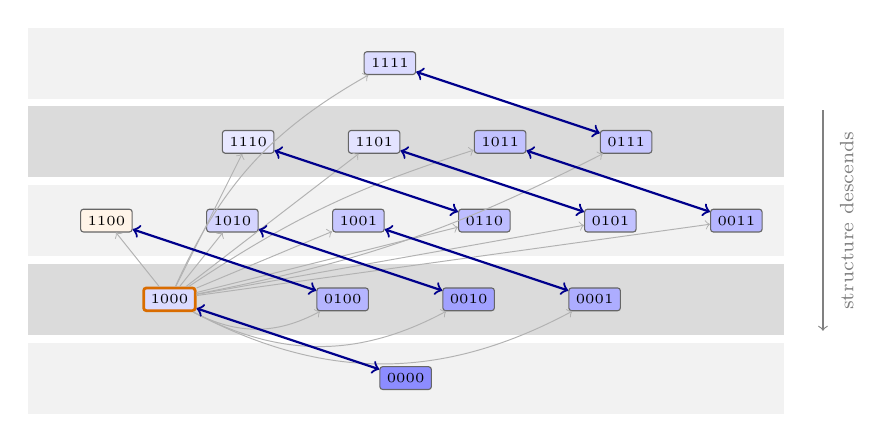
\begin{tikzpicture}[x=1cm, y=1cm,
  lnode/.style={draw=black!60, rounded corners=1pt,
                inner sep=2.5pt, font=\tiny, align=center},
  pair/.style={<->, blue!55!black, line width=0.8pt},
  denom/.style={->, gray!60, line width=0.35pt}]
  % alternating shell bands, odd shells darker
  \fill[gray!28] (-0.3,0.55) rectangle (9.3,1.45);
  \fill[gray!10] (-0.3,1.55) rectangle (9.3,2.45);
  \fill[gray!28] (-0.3,2.55) rectangle (9.3,3.45);
  \fill[gray!10] (-0.3,3.55) rectangle (9.3,4.45);
  \fill[gray!10] (-0.3,-0.45) rectangle (9.3,0.45);
  % nodes: fill hue = sign, intensity = |chi| of the prior ledger
  % shell 4
  \node[lnode, fill=blue!14] (n1111) at (4.3,4) {1111};
  % shell 3
  \node[lnode, fill=blue!9]  (n1110) at (2.5,3) {1110};
  \node[lnode, fill=blue!11] (n1101) at (4.1,3) {1101};
  \node[lnode, fill=blue!24] (n1011) at (5.7,3) {1011};
  \node[lnode, fill=blue!22] (n0111) at (7.3,3) {0111};
  % shell 2
  \node[lnode, fill=orange!9] (n1100) at (0.7,2) {1100};
  \node[lnode, fill=blue!17]  (n1010) at (2.3,2) {1010};
  \node[lnode, fill=blue!22]  (n1001) at (3.9,2) {1001};
  \node[lnode, fill=blue!26]  (n0110) at (5.5,2) {0110};
  \node[lnode, fill=blue!24]  (n0101) at (7.1,2) {0101};
  \node[lnode, fill=blue!29]  (n0011) at (8.7,2) {0011};
  % shell 1
  \node[lnode, fill=blue!14, draw=orange!85!black, line width=1pt]
    (n1000) at (1.5,1) {1000};
  \node[lnode, fill=blue!29] (n0100) at (3.7,1) {0100};
  \node[lnode, fill=blue!37] (n0010) at (5.3,1) {0010};
  \node[lnode, fill=blue!32] (n0001) at (6.9,1) {0001};
  % shell 0
  \node[lnode, fill=blue!45] (n0000) at (4.5,0) {0000};
  % the asked bias renormalizes every update: a fan from 1000
  \draw[denom] (n1000) to (n1100);
  \draw[denom] (n1000) to (n1010);
  \draw[denom] (n1000) to (n1001);
  \draw[denom] (n1000) to (n0110);
  \draw[denom] (n1000) to (n0101);
  \draw[denom] (n1000) to (n0011);
  \draw[denom] (n1000) to (n1110);
  \draw[denom] (n1000) to (n1101);
  \draw[denom, bend left=8] (n1000) to (n1011);
  \draw[denom, bend right=8] (n1000) to (n0111);
  \draw[denom, bend left=18] (n1000) to (n1111);
  \draw[denom, bend right=28] (n1000) to (n0100);
  \draw[denom, bend right=28] (n1000) to (n0010);
  \draw[denom, bend right=28] (n1000) to (n0001);
  % the eight partner pairs under toggling of 11
  \draw[pair] (n1000) -- (n0000);
  \draw[pair] (n1100) -- (n0100);
  \draw[pair] (n1010) -- (n0010);
  \draw[pair] (n1001) -- (n0001);
  \draw[pair] (n1110) -- (n0110);
  \draw[pair] (n1101) -- (n0101);
  \draw[pair] (n1011) -- (n0011);
  \draw[pair] (n1111) -- (n0111);
  % descent annotation
  \draw[->, gray] (9.8,3.4) -- (9.8,0.6);
  \node[rotate=90, gray, font=\scriptsize] at (10.1,2)
    {structure descends};
\end{tikzpicture}
\captionsetup{skip=8pt}
\captionof{figure}{The update rule in the ledger, drawn for the
guiding example's first question ($q = 11$). Every set is paired
with the partner whose membership of $11$ is toggled (arrows);
each pair is averaged with the answer's sign and renormalized,
per equation~\eqref{eq:corr-update}. The pair
$\emptyset \leftrightarrow \{11\}$ at the orange-bordered asked
set fixes the normalization and
saturates the asked bias; each blue double arrow averages a pair
into both of its members, and the net flow of structure is one
shell down, toward $M$. The thin gray arrows from the
asked $q$ to every other pill remind that this sets the
renormalization. The fill encodes each prior value to
scale: darker is larger, orange is negative.}
\label{fig:pairing}
\end{center}
\end{example}

Read formula~\eqref{eq:corr-update} by cases:
\begin{itemize}
  \item $S = \emptyset$: partner $\{q\}$, giving
    $(1 + (-1)^a \chi_{\{q\}})/(1 + (-1)^a \chi_{\{q\}}) = 1$.
    Normalization is preserved.
  \item $S = \{q\}$, the asked question: partner $\emptyset$, giving
    $(\chi_{\{q\}} + (-1)^a)/(1 + (-1)^a \chi_{\{q\}}) = (-1)^a$.
    The bias saturates to certainty --- the one-hot collapse of
    column $q$, derived rather than decreed.
  \item $S = \{q'\}$, an unasked question: the partner is the pair
    $\{q', q\}$, and one line of algebra puts the
    shift in terms of the \emph{connected} correlator:
    \begin{equation}\label{eq:cov-shift}
      \chi'_{\{q'\}} - \chi_{\{q'\}}
      \;=\; \frac{(-1)^a \big(\chi_{\{q',q\}}
        - \chi_{\{q'\}}\, \chi_{\{q\}}\big)}{2 M_{a,q}}
      \;=\; \frac{(-1)^a\, \mathrm{Cov}\big(\sigma_{q'}, \sigma_q\big)}
        {2 M_{a,q}}.
    \end{equation}
    Unasked columns move in proportion to their covariance with the
    asked question: knowledge stored one shell up descends into the
    predictions. A product prior has zero covariance everywhere, so
    its unasked columns are frozen --- the ``$C = 0$ means no
    transfer'' fact, now a one-line consequence.
  \item Higher shells: the same cascade. Each update marries
    shell-$k$ sets containing $q$ to shell-$(k{-}1)$ sets without
    it; whatever structure was stored jointly with $q$ moves one
    shell down, toward $M$.
\end{itemize}


\begin{example}
Question 1 of the walkthrough asked $q = 11$ and received $a = 1$:
sign $(-1)^a = -1$, toggled set $\{11\}$, mask $1000$.
Equation~\eqref{eq:corr-update}
maps the ledger of the previous box to
\begin{center}
\begin{tabular}{c l}
\toprule
shell & updated correlators \\
\midrule
0 & $\chi'_{0000} = 1$ \\[2pt]
1 & $\chi'_{1000} = \mathbf{-1}$,\ \ $\chi'_{0100} = +0.711$,\ \
    $\chi'_{0010} = +0.663$,\ \ $\chi'_{0001} = +0.316$ \\[2pt]
2 & $\chi'_{1100} = -0.711$,\ \ $\chi'_{1010} = -0.663$,\ \
    $\chi'_{1001} = -0.316$, \\
  & $\chi'_{0110} = +0.566$,\ \ $\chi'_{0101} = +0.412$,\ \
    $\chi'_{0011} = +0.171$ \\[2pt]
3 & $\chi'_{1110} = -0.566$,\ \ $\chi'_{1101} = -0.412$,\ \
    $\chi'_{1011} = -0.171$,\ \ $\chi'_{0111} = +0.267$ \\[2pt]
4 & $\chi'_{1111} = -0.267$ \\
\bottomrule
\end{tabular}
\end{center}
\ledgerbars{0/1/0000/blue!45,
  0.80/-1/1000/orange!80, 1.35/0.711/0100/blue!45,
  1.90/0.663/0010/blue!45, 2.45/0.316/0001/blue!45,
  3.25/-0.711/1100/orange!80, 3.80/-0.663/1010/orange!80,
  4.35/-0.316/1001/orange!80, 4.90/0.566/0110/blue!45,
  5.45/0.412/0101/blue!45, 6.00/0.171/0011/blue!45,
  6.80/-0.566/1110/orange!80, 7.35/-0.412/1101/orange!80,
  7.90/-0.171/1011/orange!80, 8.45/0.267/0111/blue!45,
  9.25/-0.267/1111/orange!80}
The asked bias saturates:
$\chi'_{1000} = (0.170 - 1)/(1 - 0.170) = -1$. The other
singletons move by equation~\eqref{eq:cov-shift}: for $q' = 10$ the
covariance is $-0.032 - (0.558)(0.170) = -0.127$, so the shift is
$(-1)(-0.127)/(2 \times 0.415) = +0.153$, landing on $+0.711$ ---
and indeed $(1 + 0.711)/2 = 0.855$, the column $M_{0,10}$ of the
Question 2 box. Note also that every mask containing the asked bit
is now just $(-1)^a$ times its partner
($\chi'_{1010} = -\chi'_{0010}$,
etc.): with $\sigma_{11}$ pinned, no correlator involving
question $11$ carries independent knowledge anymore.

\begin{center}
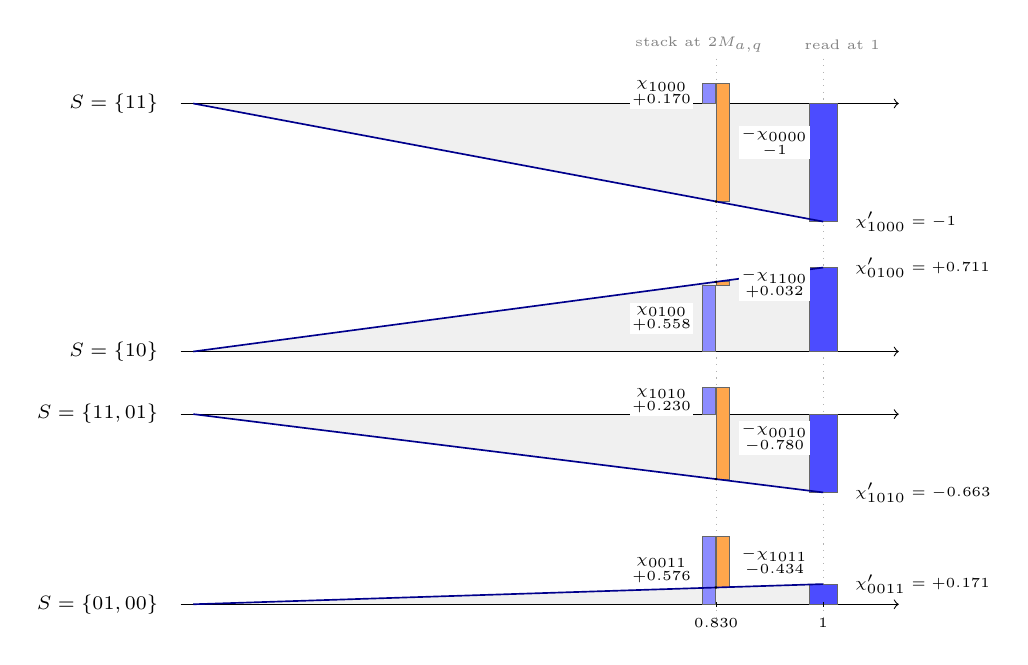
\begin{tikzpicture}[x=8cm, y=1.5cm]
  % the update rule (eq:corr-update), drawn: per set S, the numerator
  % chi_S with the twin's signed contribution beside it (waterfall)
  % at x = 2M_{a,q}, rescaled to x = 1 by the ray through the origin
  \draw[dotted, gray!60] (0.830,0.38) -- (0.830,-4.35);
  \draw[dotted, gray!60] (1,0.38) -- (1,-4.35);
  % \node[font=\small\itshape] at (0.5,0.85)
  %   {update $\chi$ after $\psi(11) = 1$};
  \node[font=\tiny, gray, anchor=east] at (0.92,0.50)
    {stack at $2M_{a,q}$};
  \node[font=\tiny, gray, anchor=west] at (0.955,0.50)
    {read at $1$};
  % the set being updated, left of each row
  \node[font=\scriptsize, anchor=east] at (-0.04,0)
    {$S = \{11\}$};
  \node[font=\scriptsize, anchor=east] at (-0.04,-2.1)
    {$S = \{10\}$};
  \node[font=\scriptsize, anchor=east] at (-0.04,-2.63)
    {$S = \{11, 01\}$};
  \node[font=\scriptsize, anchor=east] at (-0.04,-4.24)
    {$S = \{01, 00\}$};
  % ---------- S = 1000 (the asked set) ----------
  \fill[gray!12] (0,0) -- (1,0) -- (1,-1) -- cycle;
  \draw[->] (-0.02,0) -- (1.12,0);
  \draw[fill=blue!45, draw=black!60, line width=0.3pt]
    (0.809,0) rectangle (0.829,0.170);
  \draw[fill=orange!70, draw=black!60, line width=0.3pt]
    (0.831,0.170) rectangle (0.851,-0.830);
  \draw[fill=blue!70, draw=black!60, line width=0.3pt]
    (0.978,0) rectangle (1.022,-1);
  \draw[blue!55!black, line width=0.6pt] (0,0) -- (1,-1);
  \fill[black] (0.830,-0.830) circle (0.5pt);
  \node[font=\tiny, fill=white, inner sep=1pt, anchor=east,
    align=center] at (0.795,0.085) {$\chi_{1000}$\\$+0.170$};
  \node[font=\tiny, fill=white, inner sep=1pt, anchor=west,
    align=center] at (0.865,-0.33) {$-\chi_{0000}$\\$-1$};
  \node[font=\tiny, anchor=west, align=center] at (1.035,-1)
    {$\chi'_{1000} = -1$};
  % ---------- S = 0100 (an unasked question) ----------
  \fill[gray!12] (0,-2.1) -- (1,-2.1) -- (1,-1.389) -- cycle;
  \draw[->] (-0.02,-2.1) -- (1.12,-2.1);
  \draw[fill=blue!45, draw=black!60, line width=0.3pt]
    (0.809,-2.1) rectangle (0.829,-1.542);
  \draw[fill=orange!70, draw=black!60, line width=0.3pt]
    (0.831,-1.542) rectangle (0.851,-1.510);
  \draw[fill=blue!70, draw=black!60, line width=0.3pt]
    (0.978,-2.1) rectangle (1.022,-1.389);
  \draw[blue!55!black, line width=0.6pt] (0,-2.1) -- (1,-1.389);
  \fill[black] (0.830,-1.510) circle (0.5pt);
  \node[font=\tiny, fill=white, inner sep=1pt, anchor=east,
    align=center] at (0.795,-1.821) {$\chi_{0100}$\\$+0.558$};
  \node[font=\tiny, fill=white, inner sep=1pt, anchor=west,
    align=center] at (0.865,-1.526) {$-\chi_{1100}$\\$+0.032$};
  \node[font=\tiny, anchor=west, align=center] at (1.035,-1.389)
    {$\chi'_{0100} = +0.711$};
  % ---------- S = 1010 (contains the asked bit) ----------
  \fill[gray!12] (0,-2.63) -- (1,-2.63) -- (1,-3.293) -- cycle;
  \draw[->] (-0.02,-2.63) -- (1.12,-2.63);
  \draw[fill=blue!45, draw=black!60, line width=0.3pt]
    (0.809,-2.63) rectangle (0.829,-2.40);
  \draw[fill=orange!70, draw=black!60, line width=0.3pt]
    (0.831,-2.40) rectangle (0.851,-3.18);
  \draw[fill=blue!70, draw=black!60, line width=0.3pt]
    (0.978,-2.63) rectangle (1.022,-3.293);
  \draw[blue!55!black, line width=0.6pt] (0,-2.63) -- (1,-3.293);
  \fill[black] (0.830,-3.18) circle (0.5pt);
  \node[font=\tiny, fill=white, inner sep=1pt, anchor=east,
    align=center] at (0.795,-2.515) {$\chi_{1010}$\\$+0.230$};
  \node[font=\tiny, fill=white, inner sep=1pt, anchor=west,
    align=center] at (0.865,-2.83) {$-\chi_{0010}$\\$-0.780$};
  \node[font=\tiny, anchor=west, align=center] at (1.035,-3.293)
    {$\chi'_{1010} = -0.663$};
  % ---------- S = 0011 (a higher shell) ----------
  \fill[gray!12] (0,-4.24) -- (1,-4.24) -- (1,-4.069) -- cycle;
  \draw[->] (-0.02,-4.24) -- (1.12,-4.24);
  \draw[fill=blue!45, draw=black!60, line width=0.3pt]
    (0.809,-4.24) rectangle (0.829,-3.664);
  \draw[fill=orange!70, draw=black!60, line width=0.3pt]
    (0.831,-3.664) rectangle (0.851,-4.098);
  \draw[fill=blue!70, draw=black!60, line width=0.3pt]
    (0.978,-4.24) rectangle (1.022,-4.069);
  \draw[blue!55!black, line width=0.6pt] (0,-4.24) -- (1,-4.069);
  \fill[black] (0.830,-4.098) circle (0.5pt);
  \node[font=\tiny, fill=white, inner sep=1pt, anchor=east,
    align=center] at (0.795,-3.952) {$\chi_{0011}$\\$+0.576$};
  \node[font=\tiny, fill=white, inner sep=1pt, anchor=west,
    align=center] at (0.865,-3.881) {$-\chi_{1011}$\\$-0.434$};
  \node[font=\tiny, anchor=west, align=center] at (1.035,-4.069)
    {$\chi'_{0011} = +0.171$};
  % shared x labels on the bottom panel
  \draw (0.830,-4.26) -- (0.830,-4.22);
  \draw (1,-4.26) -- (1,-4.22);
  \node[font=\tiny, below] at (0.830,-4.28) {$0.830$};
  \node[font=\tiny, below] at (1,-4.28) {$1$};
\end{tikzpicture}
\captionsetup{skip=8pt}
\captionof{figure}{The update rule of
equation~\eqref{eq:corr-update}, drawn for the guiding example's
first update ($q = 11$, $a = 1$, so $(-1)^a = -1$ and toggled bit
$1000$). One row per set $S$. At $x = 2M_{a,q} = 1 + (-1)^a
\chi_{1000} = 0.830$ stands the numerator as a waterfall: the bar
of $\chi_S$ (blue), and beside it the partner's signed
contribution $(-1)^a \chi_{S \triangle \{q\}}$ (orange), hanging
from the level where the first bar ends. The two subscripts
differ by the flipped bit. The ray from the origin through the
waterfall's endpoint rescales it, by similar triangles, to
$x = 1$, where its height is the updated correlator $\chi'_S$.}
\label{fig:update-rays}
\end{center}
\end{example}

As Werner moves through the questions, more correlators settle to $\pm 1$. The 1-shell models the belief of the bias of each question. 
The 2-shell answers questions such as 'If the answer to $\psi(10) = 0$, then $\psi(01) = 1$'. And the higher orders are even more conditional, measuring belief about such statements, in the case of certain answers, etc. As we learn more, the conditions become satisfied or not, and the information becomes less nested. 

\begin{example}
The remaining
questions of the run ($00$, $01$, $10$, all answered $0$, so with
sign $+1$) each saturate their own bit the same way, and since
XOR toggles commute, the order does not matter --- the
commutativity of updating, seen again. After all four, the ledger
is pure signs, $\chi_S = (-1)^{|S \cap \{11\}|}$ --- $-1$ on every
set containing $11$, $+1$ on the rest: the transform
of the point mass on $\psi = \phi_8$:
\begin{center}
\begin{tabular}{c l}
\toprule
shell & final correlators \\
\midrule
0 & $\chi_{0000} = 1$ \\[2pt]
1 & $\chi_{1000} = -1$,\ \ $\chi_{0100} = +1$,\ \
    $\chi_{0010} = +1$,\ \ $\chi_{0001} = +1$ \\[2pt]
2 & $\chi_{1100} = -1$,\ \ $\chi_{1010} = -1$,\ \
    $\chi_{1001} = -1$, \\
  & $\chi_{0110} = +1$,\ \ $\chi_{0101} = +1$,\ \
    $\chi_{0011} = +1$ \\[2pt]
3 & $\chi_{1110} = -1$,\ \ $\chi_{1101} = -1$,\ \
    $\chi_{1011} = -1$,\ \ $\chi_{0111} = +1$ \\[2pt]
4 & $\chi_{1111} = -1$ \\
\bottomrule
\end{tabular}
\end{center}
\ledgerbars{0/1/0000/blue!45,
  0.80/-1/1000/orange!80, 1.35/1/0100/blue!45,
  1.90/1/0010/blue!45, 2.45/1/0001/blue!45,
  3.25/-1/1100/orange!80, 3.80/-1/1010/orange!80,
  4.35/-1/1001/orange!80, 4.90/1/0110/blue!45,
  5.45/1/0101/blue!45, 6.00/1/0011/blue!45,
  6.80/-1/1110/orange!80, 7.35/-1/1101/orange!80,
  7.90/-1/1011/orange!80, 8.45/1/0111/blue!45,
  9.25/-1/1111/orange!80}
\end{example}

\subsection{General $m$}\label{sec:generalm}

It turns out that taking $m > 1$ is more
general but not much more instructive. With multiple output bits it
is as if we have $m$ a priori independent maps per question; they
just happen always to be asked and answered simultaneously, in
unison. Therefore we do not have to think about what one of them
teaches us about another. It would mean we have more than $2$
options every question, and therefore the factor by which every
update thins the hypotheses is not $2$ but $2^m$. The guiding
example helps because the maps are represented as binary numbers,
which are more familiar.

For completeness, the main formulas. The truth table is now
$m \cdot 2^n$ bits: one \emph{site} $(q, i)$ per bit $i$ of each
answer, each carrying a spin
$\sigma_{q,i}(\phi_j) := (-1)^{\phi_j(q)_i}$, where $\phi_j(q)_i$
is the $i$-th bit of the answer. Correlators are indexed by sets
$S$ of sites --- masks of $m 2^n$ bits under the same numeral
convention, $m$ of them per question:
\begin{equation}\label{eq:wht-m}
  \chi_S \;=\; \Big\langle \prod_{(q,i) \in S} \sigma_{q,i}
  \Big\rangle
  \;=\; \sum_{j=0}^{N-1} (-1)^{\sum_{(q,i) \in S} \phi_j(q)_i}\,
  p_j.
\end{equation}

\begin{example}
For $n = 3$, $m = 2$ the sites form a $2 \times 8$ grid: one column
per question, one row per bit of the answer. A set $S$ is a pattern
of hot cells in this grid, and $\chi_S$ multiplies the
corresponding spins:
\begin{center}
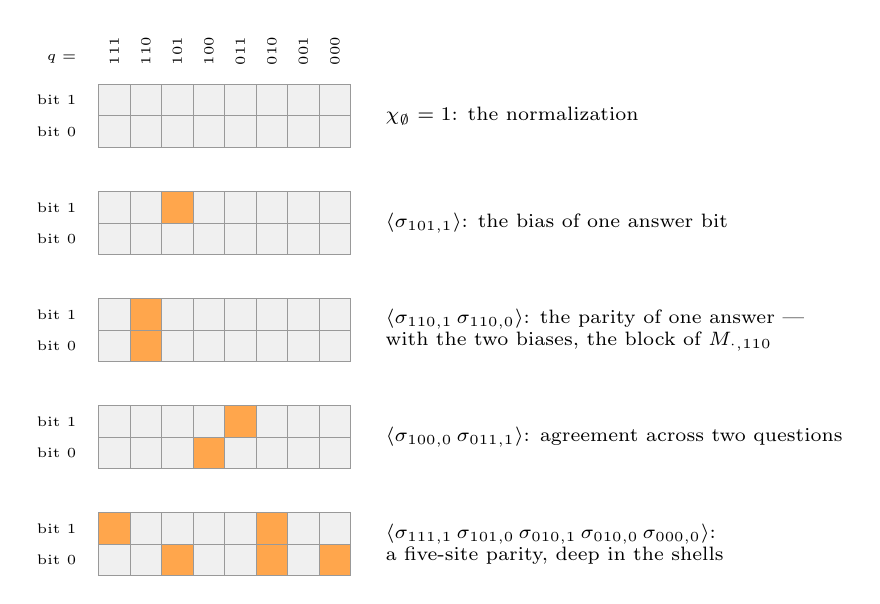
\begin{tikzpicture}[x=0.40cm, y=0.40cm]
  % column headers
  \node[font=\tiny, anchor=east] at (-0.4,0.8) {$q =$};
  \foreach \c/\q in {0/111, 1/110, 2/101, 3/100,
                     4/011, 5/010, 6/001, 7/000}
    \node[font=\tiny, rotate=90, anchor=west] at ({\c+0.5},0.3)
      {$\q$};
  % row labels, all grids
  \foreach \g in {0, 1, 2, 3, 4} {
    \node[font=\tiny, anchor=east] at (-0.4,{-3.4*\g - 0.5})
      {bit $1$};
    \node[font=\tiny, anchor=east] at (-0.4,{-3.4*\g - 1.5})
      {bit $0$};
  }
  % the five grids: cold cells
  \foreach \g in {0, 1, 2, 3, 4}
    \foreach \c in {0,...,7}
      \foreach \r in {0, 1}
        \draw[black!40, line width=0.3pt, fill=gray!12]
          (\c,{-3.4*\g - 2 + \r}) rectangle
          ({\c+1},{-3.4*\g - 1 + \r});
  % hot cells: {grid/column/row}, row 1 = bit 1 (top)
  \foreach \g/\c/\r in {1/2/1, 2/1/0, 2/1/1, 3/3/0, 3/4/1,
                        4/0/1, 4/2/0, 4/5/0, 4/5/1, 4/7/0}
    \draw[black!40, line width=0.3pt, fill=orange!70]
      (\c,{-3.4*\g - 2 + \r}) rectangle
      ({\c+1},{-3.4*\g - 1 + \r});
  % what each pattern computes
  \node[font=\scriptsize, anchor=west] at (8.8,-1)
    {$\chi_\emptyset = 1$: the normalization};
  \node[font=\scriptsize, anchor=west] at (8.8,-4.4)
    {$\langle \sigma_{101,1} \rangle$: the bias of one answer bit};
  \node[font=\scriptsize, anchor=west, align=left] at (8.8,-7.8)
    {$\langle \sigma_{110,1}\, \sigma_{110,0} \rangle$: the parity
     of one answer ---\\with the two biases, the block of
     $M_{\cdot,110}$};
  \node[font=\scriptsize, anchor=west] at (8.8,-11.2)
    {$\langle \sigma_{100,0}\, \sigma_{011,1} \rangle$: agreement
     across two questions};
  \node[font=\scriptsize, anchor=west, align=left] at (8.8,-14.6)
    {$\langle \sigma_{111,1}\, \sigma_{101,0}\, \sigma_{010,1}\,
      \sigma_{010,0}\, \sigma_{000,0} \rangle$:\\a five-site
      parity, deep in the shells};
\end{tikzpicture}
\end{center}
Any of the $2^{16} = 65536$ hot/cold patterns is a correlator, and
sorting by the number of hot cells gives the shells. The mask of
$S$ is the grid read as a $16$-bit numeral.
\end{example}

Write $B_q$ for the block of $q$'s $m$ sites, and
$a \cdot T := \sum_{i \in T} a_i$ for the parity of the answer $a$
on a subset $T \subseteq B_q$. The answer matrix is read off the
correlators supported on one block --- $2^m$ of them per column:
\begin{equation}\label{eq:M-m}
  M_{a,q} \;=\; \frac{1}{2^m} \sum_{T \subseteq B_q}
  (-1)^{a \cdot T}\, \chi_T.
\end{equation}
The observation mask at $(q, a)$ is a function of the $m$ bits of
one block, so its ledger has $2^m$ nonzero entries, and hearing
$a = \psi(q)$ combines every correlator with its $2^m$ partners ---
one per toggle $T$ within the asked block:
\begin{equation}\label{eq:corr-update-m}
  \chi'_S \;=\; \frac{\sum_{T \subseteq B_q} (-1)^{a \cdot T}\,
    \chi_{S \triangle T}}{2^m\, M_{a,q}},
\end{equation}
the denominator once more the $S = \emptyset$ instance of the
numerator. For $m = 1$ the three
formulas collapse to
equations~\eqref{eq:wht}, \eqref{eq:shell1}
and~\eqref{eq:corr-update}.

\begin{example}
To draw the update, take a sparse prior at $n = 3$, $m = 2$: four
maps, $\phi(q) = q \bmod 4$ (weight $0.45$), constant $00$
($0.35$), ``$11$ iff $q \geq 4$'' ($0.12$), constant $11$
($0.08$). Werner asks $q = 110$ and hears $a = 11$: toggle signs
$(+, -, -, +)$ on $(\emptyset, 110_0, 110_1, \text{both})$, where
$q_i$ denotes site $(q, i)$, and denominator
$2^m M_{11,110} = 0.8$. The pairs of the $m = 1$ figure become
\emph{quartets}:
\begin{center}
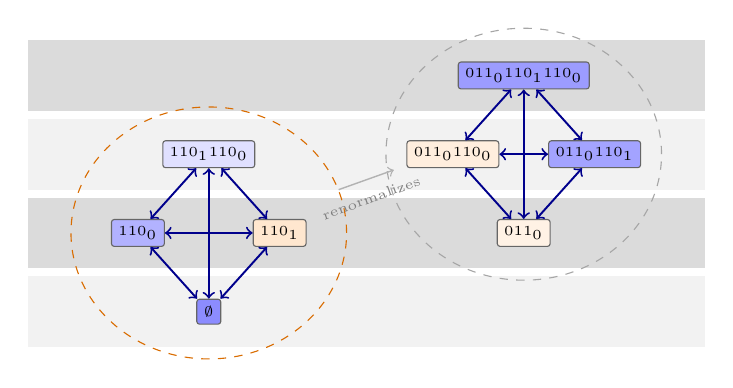
\begin{tikzpicture}[x=1cm, y=1cm,
  lnode/.style={draw=black!60, rounded corners=1pt,
                inner sep=2.5pt, font=\tiny, align=center},
  pair/.style={<->, blue!55!black, line width=0.7pt}]
  % shell bands, odd darker
  \fill[gray!10] (-0.3,-0.45) rectangle (8.3,0.45);
  \fill[gray!28] (-0.3,0.55) rectangle (8.3,1.45);
  \fill[gray!10] (-0.3,1.55) rectangle (8.3,2.45);
  \fill[gray!28] (-0.3,2.55) rectangle (8.3,3.45);
  % the on-block quartet of the asked question 110
  \node[lnode, fill=blue!45]  (qa0) at (2,0)   {$\emptyset$};
  \node[lnode, fill=blue!30]  (qa1) at (1.1,1) {$110_0$};
  \node[lnode, fill=orange!19] (qa2) at (2.9,1) {$110_1$};
  \node[lnode, fill=blue!12]  (qa3) at (2,2)   {$110_1 110_0$};
  \draw[pair] (qa0) -- (qa1); \draw[pair] (qa0) -- (qa2);
  \draw[pair] (qa0) -- (qa3); \draw[pair] (qa1) -- (qa2);
  \draw[pair] (qa1) -- (qa3); \draw[pair] (qa2) -- (qa3);
  % a generic quartet, seeded by the foreign site 011_0
  \node[lnode, fill=orange!10] (qb0) at (6,1)   {$011_0$};
  \node[lnode, fill=orange!13] (qb1) at (5.1,2) {$011_0 110_0$};
  \node[lnode, fill=blue!36]   (qb2) at (6.9,2) {$011_0 110_1$};
  \node[lnode, fill=blue!39]   (qb3) at (6,3)   {$011_0 110_1 110_0$};
  \draw[pair] (qb0) -- (qb1); \draw[pair] (qb0) -- (qb2);
  \draw[pair] (qb0) -- (qb3); \draw[pair] (qb1) -- (qb2);
  \draw[pair] (qb1) -- (qb3); \draw[pair] (qb2) -- (qb3);
  % the asked block's quartet renormalizes every other
  \draw[dashed, orange!85!black] (2,1) ellipse (1.75 and 1.6);
  \draw[dashed, gray!70] (6,2) ellipse (1.75 and 1.6);
  \draw[->, gray!60, line width=0.5pt] (3.65,1.55) -- (4.35,1.8);
  \node[font=\tiny, gray, below, rotate=20] at (4.0,1.62)
    {renormalizes};
\end{tikzpicture}
\captionsetup{skip=8pt}
\captionof{figure}{For $m = 2$, toggling any subset of the asked
block's two sites ties four correlators into a clique that
averages jointly, per equation~\eqref{eq:corr-update-m}. The
on-block quartet (orange hull) contains the normalization and the
entire block of $M_{\cdot,110}$; its signed sum is the denominator
that renormalizes every other quartet. Fills to scale for the
sparse prior, as before.}
\label{fig:quartets}

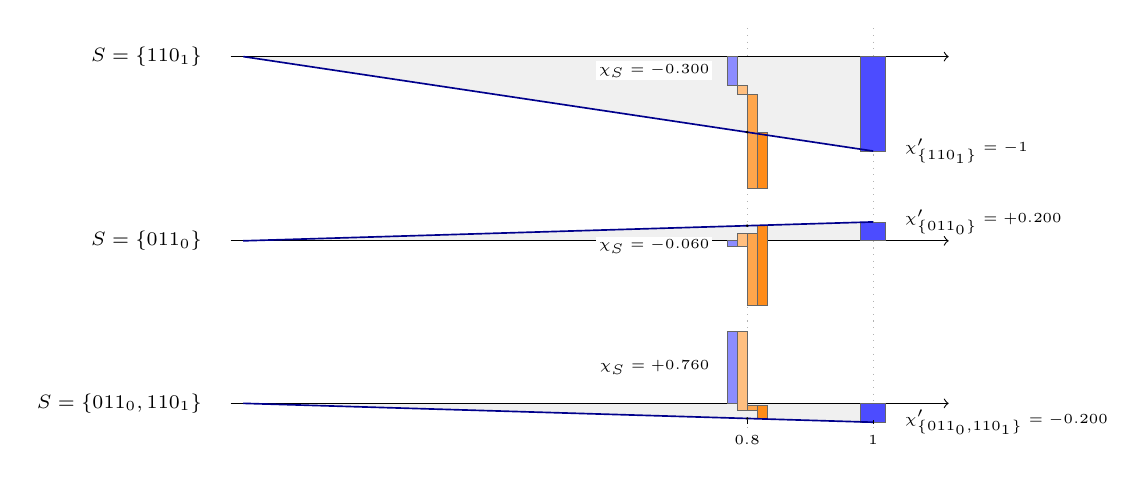
\begin{tikzpicture}[x=8cm, y=1.2cm]
  % \node[font=\small\itshape] at (0.5,0.55)
  %   {update $\chi$ after $\psi(110) = 11$};
  \draw[dotted, gray!60] (0.8,0.3) -- (0.8,-3.95);
  \draw[dotted, gray!60] (1,0.3) -- (1,-3.95);
  % ---------- S = {110_1} ----------
  \fill[gray!12] (0,0) -- (1,0) -- (1,-1) -- cycle;
  \draw[->] (-0.02,0) -- (1.12,0);
  \draw[fill=blue!45, draw=black!60, line width=0.3pt]
    (0.768,0) rectangle (0.784,-0.300);
  \draw[fill=orange!50, draw=black!60, line width=0.3pt]
    (0.784,-0.300) rectangle (0.800,-0.400);
  \draw[fill=orange!70, draw=black!60, line width=0.3pt]
    (0.800,-0.400) rectangle (0.816,-1.400);
  \draw[fill=orange!90, draw=black!60, line width=0.3pt]
    (0.816,-1.400) rectangle (0.832,-0.800);
  \draw[fill=blue!70, draw=black!60, line width=0.3pt]
    (0.98,0) rectangle (1.02,-1);
  \draw[blue!55!black, line width=0.6pt] (0,0) -- (1,-1);
  \fill[black] (0.8,-0.8) circle (0.5pt);
  \node[font=\tiny, fill=white, inner sep=1pt, anchor=east]
    at (0.745,-0.15) {$\chi_S = -0.300$};
  \node[font=\tiny, anchor=west] at (1.035,-1)
    {$\chi'_{\{110_1\}} = -1$};
  \node[font=\scriptsize, anchor=east] at (-0.05,0)
    {$S = \{110_1\}$};
  % ---------- S = {011_0} ----------
  \fill[gray!12] (0,-1.95) -- (1,-1.95) -- (1,-1.75) -- cycle;
  \draw[->] (-0.02,-1.95) -- (1.12,-1.95);
  \draw[fill=blue!45, draw=black!60, line width=0.3pt]
    (0.768,-1.95) rectangle (0.784,-2.010);
  \draw[fill=orange!50, draw=black!60, line width=0.3pt]
    (0.784,-2.010) rectangle (0.800,-1.870);
  \draw[fill=orange!70, draw=black!60, line width=0.3pt]
    (0.800,-1.870) rectangle (0.816,-2.630);
  \draw[fill=orange!90, draw=black!60, line width=0.3pt]
    (0.816,-2.630) rectangle (0.832,-1.790);
  \draw[fill=blue!70, draw=black!60, line width=0.3pt]
    (0.98,-1.95) rectangle (1.02,-1.75);
  \draw[blue!55!black, line width=0.6pt] (0,-1.95) -- (1,-1.75);
  \fill[black] (0.8,-1.79) circle (0.5pt);
  \node[font=\tiny, fill=white, inner sep=1pt, anchor=east]
    at (0.745,-2.01) {$\chi_S = -0.060$};
  \node[font=\tiny, anchor=west] at (1.035,-1.75)
    {$\chi'_{\{011_0\}} = +0.200$};
  \node[font=\scriptsize, anchor=east] at (-0.05,-1.95)
    {$S = \{011_0\}$};
  % ---------- S = {011_0, 110_1} ----------
  \fill[gray!12] (0,-3.67) -- (1,-3.67) -- (1,-3.87) -- cycle;
  \draw[->] (-0.02,-3.67) -- (1.12,-3.67);
  \draw[fill=blue!45, draw=black!60, line width=0.3pt]
    (0.768,-3.67) rectangle (0.784,-2.910);
  \draw[fill=orange!50, draw=black!60, line width=0.3pt]
    (0.784,-2.910) rectangle (0.800,-3.750);
  \draw[fill=orange!70, draw=black!60, line width=0.3pt]
    (0.800,-3.750) rectangle (0.816,-3.690);
  \draw[fill=orange!90, draw=black!60, line width=0.3pt]
    (0.816,-3.690) rectangle (0.832,-3.830);
  \draw[fill=blue!70, draw=black!60, line width=0.3pt]
    (0.98,-3.67) rectangle (1.02,-3.87);
  \draw[blue!55!black, line width=0.6pt] (0,-3.67) -- (1,-3.87);
  \fill[black] (0.8,-3.83) circle (0.5pt);
  \node[font=\tiny, fill=white, inner sep=1pt, anchor=east]
    at (0.745,-3.29) {$\chi_S = +0.760$};
  \node[font=\tiny, anchor=west] at (1.035,-3.87)
    {$\chi'_{\{011_0, 110_1\}} = -0.200$};
  \node[font=\scriptsize, anchor=east] at (-0.05,-3.67)
    {$S = \{011_0, 110_1\}$};
  % shared x labels
  \draw (0.8,-3.89) -- (0.8,-3.85);
  \draw (1,-3.89) -- (1,-3.85);
  \node[font=\tiny, below] at (0.8,-3.91) {$0.8$};
  \node[font=\tiny, below] at (1,-3.91) {$1$};
\end{tikzpicture}
\captionsetup{skip=8pt}
\captionof{figure}{The $m = 2$ update, three sets from the sparse
prior. The waterfall now has four segments: $\chi_S$ (blue) and
its three signed quartet partners, in toggle order $110_0$,
$110_1$, both (light to dark orange). The ray from the origin
rescales the endpoint from $x = 2^m M_{a,q} = 0.8$ to $x = 1$.
The asked site saturates to $-1$; the foreign site $011_0$ flips
sign, $-0.060 \to +0.200$; and $\{011_0, 110_1\}$ lands on
$-0.200$, the slaved value $-\chi'_{\{011_0\}}$.}
\label{fig:update-rays-m2}
\end{center}
\end{example}

\section{Expectations}\label{sec:expectations}

In expectation over the truth $\psi \sim p$, as well as over the question order, we take the ratio of
the expected totals,
\begin{equation}\label{eq:Lk-avg}
  \langle L_\ell \rangle \;:=\;
  \frac{H\big(M^{(0)}\big) - \big\langle  H\big(M^{(\ell)}\big) \big\rangle}
       {\big\langle \sum_{i=1}^{\ell} s_i \big\rangle}\;.
\end{equation}

We did this implicitly in
Section~\ref{sec:oneparam}. There, the problem was actually symmetric in $q_0 \leftrightarrow q_1$. That is not the case in general.

In order to progress, we will be interested in such averages. Both
are natural. The question order is uniform, without replacement:
before any evidence arrives, there is no reason to prefer one
question over another. And the truth is drawn from the prior
itself: Werner scores his future against his own beliefs, and he
has faith in them.

The bookkeeping simplifies at once. Updating commutes, so after
$\ell$ rounds the state depends only on the asked \emph{set} $S$,
a uniform random subset of size $\ell$. And the received
surprisals telescope to the surprisal of the whole answer block,
\begin{equation}\label{eq:telescope}
  \sum_{i=1}^{\ell} s_i \;=\; -\log_2 P\big(A_S = \psi(S)\big),
\end{equation}
whose average over $\psi$ is a block entropy. Everything is
therefore generated by one sequence, the mean block entropy at
size $k$:
\begin{equation}\label{eq:Gk}
  G_k \;:=\; \binom{2^n}{k}^{-1} \sum_{|S| = k} H(A_S),
  \qquad G_0 = 0, \qquad G_{2^n} = H(p).
\end{equation}
$G_1$ is the mean column entropy, so $H(M)_0 = 2^n G_1$. Two
exact laws follow. The first is
equation~\eqref{eq:telescope} averaged:
\begin{equation}\label{eq:law-received}
  \Big\langle \sum_{i=1}^{\ell} s_i \Big\rangle \;=\; G_\ell.
\end{equation}
For the second, fix $S$ and average the posterior table over the
answers. Each unasked column's entropy becomes a conditional
entropy, $H(A_{q'} \mid A_S) = H(A_{S \cup \{q'\}}) - H(A_S)$,
and the asked columns contribute zero. Now average over $S$:
every set of size $\ell + 1$ arises as $S \cup \{q'\}$ once per
element, and counting with
$(\ell{+}1)\binom{2^n}{\ell+1} = (2^n{-}\ell)\binom{2^n}{\ell}$,
\begin{equation}\label{eq:law-remaining}
  \big\langle H\big(M^{(\ell)}\big) \big\rangle
  \;=\; (2^n - \ell)\,\big(G_{\ell+1} - G_\ell\big).
\end{equation}
The whole expected learning curve is the discrete derivative of
one monotone sequence. By conservation, destruction and deduction
are the differences $H(M)_0 - \langle H(M^{(\ell)}) \rangle$ and
$H(M)_0 - \langle H(M^{(\ell)}) \rangle - G_\ell$, and
equation~\eqref{eq:Lk-avg} becomes
\begin{equation}\label{eq:Lk-G}
  \langle L_\ell \rangle \;=\;
  \frac{H(M)_0 - (2^n - \ell)\big(G_{\ell+1} - G_\ell\big)}
       {G_\ell}\;.
\end{equation}
In terms of the prior, the block entropies are explicit. The maps
that answer the pattern $b$ on the asked set $S$ form a residue
class, with mass
\begin{equation}\label{eq:Gk-pj}
  G_\ell \;=\; -\binom{2^n}{\ell}^{-1} \sum_{|S| = \ell}\;
  \sum_{b} P_{S,b} \log_2 P_{S,b},
  \qquad
  P_{S,b} \;:=\; \sum_{j \,:\, \phi_j(q) = b_q \;\forall q \in S}
  p_j,
\end{equation}
the inner sum running over the $2^\ell$ answer patterns $b$ on
$S$. Nothing here is specific to $m = 1$: blocks of $m$-bit
answers obey the same laws verbatim, with $b$ running over the
$(2^m)^\ell$ patterns of the block.

Some observations.
\begin{itemize}
  \item Expectation kills the windfall. Each step has
    $\langle \Delta H(p) - s \rangle = 0$, so the expected deduced
    part is a pure tower withdrawal:
    $H(M)_0 - \langle H(M^{(\ell)}) \rangle - G_\ell
    = C_0 - \langle C_\ell \rangle$, with
    $\langle C_\ell \rangle =
    \langle H(M^{(\ell)}) \rangle - \big(H(p) - G_\ell\big)$. It
    is nonnegative: anti-leverage is only ever bad luck.
  \item Deduction saturates one round early: substituting
    $G_{2^n} = H(p)$ at $\ell = 2^n - 1$ already gives
    $\langle C_{2^n - 1} \rangle = 0$. The store is empty before
    the last question, which can only be observed, never
    leveraged.
  \item $\langle L_\ell \rangle \geq 1$ always, but it need not be
    monotone. The endpoint is forced:
    $\langle L_{2^n} \rangle = H(M)_0 / H(p) = 1 + C_0/H(p)$, the
    run ratio quoted in Section~\ref{sec:general}. This is also
    why equation~\eqref{eq:Lk-avg} is a ratio of expectations: the
    expectation of the ratio is dominated by lucky runs with
    vanishing denominators.
  \item Sanity: $\ell = 0$ returns $H(M)_0 = 2^n G_1$, and at
    $n = 1$ the laws reproduce the one-parameter world of
    Section~\ref{sec:oneparam}.
\end{itemize}

There is also a monotonicity theorem hiding in $G$. Entropy is
submodular, so the increments $G_\ell - G_{\ell-1}$, which are
the expected surprisals of the $\ell$-th answer, decrease with
$\ell$: answers get cheaper as evidence accumulates. Greedy play
does the opposite on purpose, seeking out the most expensive
question on the board.

\begin{example}
For the guiding prior the block-entropy sequence is
$G_k = (0,\ 0.731,\ 1.436,\ 2.100,\ 2.707)$, and the laws unfold
it into the expected run:
\begin{center}
\begin{tabular}{c c c c c}
\toprule
 & received & remaining & store & leverage \\
$\ell$ & $\big\langle \sum_i s_i \big\rangle$
  & $\big\langle H\big(M^{(\ell)}\big) \big\rangle$
  & $\langle C_\ell \rangle$
  & $\langle L_\ell \rangle$ \\
\midrule
1 & 0.731 & 2.113 & 0.137 & 1.110 \\
2 & 1.436 & 1.328 & 0.056 & 1.113 \\
3 & 2.100 & 0.608 & 0     & 1.104 \\
4 & 2.707 & 0     & 0     & 1.081 \\
\bottomrule
\end{tabular}
\end{center}
The expected leverage humps at $\ell = 2$ and lands on
$2.925/2.707 = 1.081$. The realized run of
Section~\ref{sec:general} scattered around this gentle
expectation: greedy questioning and a lucky truth delivered
$1.311$. Figure~\ref{fig:expected-stack} stacks the expected
books.

\begin{center}
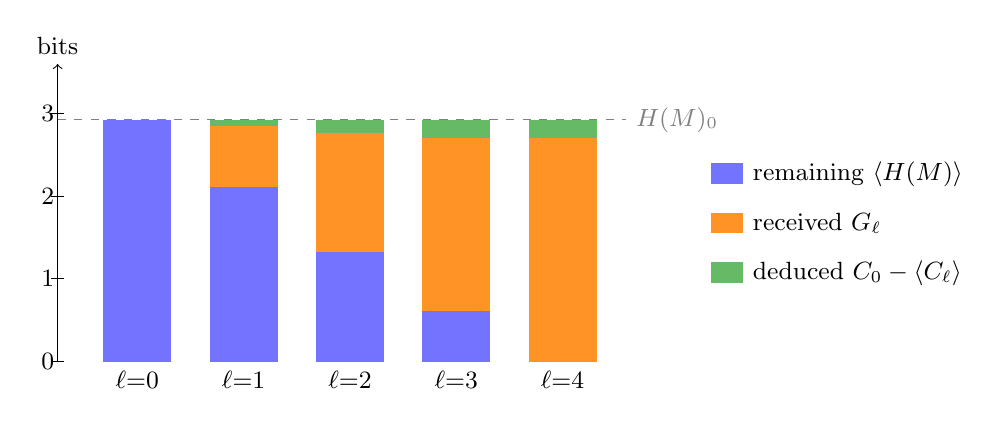
\begin{tikzpicture}[x=1.35cm, y=1.05cm]
  % axis
  \draw[->] (-0.75,0) -- (-0.75,3.6);
  \node[above, font=\small] at (-0.75,3.6) {bits};
  \foreach \y in {0,1,2,3}
    \draw (-0.81,\y) -- (-0.69,\y) node[left, font=\small] {$\y$};
  % l = 0
  \fill[blue!55] (-0.32,0) rectangle (0.32,2.925);
  % l = 1
  \fill[blue!55] (0.68,0) rectangle (1.32,2.113);
  \fill[orange!85] (0.68,2.113) rectangle (1.32,2.844);
  \fill[green!55!black!60] (0.68,2.844) rectangle (1.32,2.925);
  % l = 2
  \fill[blue!55] (1.68,0) rectangle (2.32,1.328);
  \fill[orange!85] (1.68,1.328) rectangle (2.32,2.764);
  \fill[green!55!black!60] (1.68,2.764) rectangle (2.32,2.925);
  % l = 3
  \fill[blue!55] (2.68,0) rectangle (3.32,0.608);
  \fill[orange!85] (2.68,0.608) rectangle (3.32,2.708);
  \fill[green!55!black!60] (2.68,2.708) rectangle (3.32,2.925);
  % l = 4
  \fill[orange!85] (3.68,0) rectangle (4.32,2.707);
  \fill[green!55!black!60] (3.68,2.707) rectangle (4.32,2.925);
  % initial-total line
  \draw[dashed, gray] (-0.75,2.925) -- (4.6,2.925);
  \node[right, font=\small, gray] at (4.6,2.925) {$H(M)_0$};
  % x labels
  \foreach \l in {0,...,4}
    \node[below, font=\small] at (\l,0) {$\ell{=}\l$};
  % legend
  \fill[blue!55] (5.4,2.15) rectangle (5.7,2.4);
  \node[right, font=\small] at (5.7,2.27)
    {remaining $\langle H(M) \rangle$};
  \fill[orange!85] (5.4,1.55) rectangle (5.7,1.8);
  \node[right, font=\small] at (5.7,1.67) {received $G_\ell$};
  \fill[green!55!black!60] (5.4,0.95) rectangle (5.7,1.2);
  \node[right, font=\small] at (5.7,1.07)
    {deduced $C_0 - \langle C_\ell \rangle$};
\end{tikzpicture}
\captionsetup{skip=8pt}
\captionof{figure}{The expected run through the guiding example.
Conservation is now exact at every $\ell$: remaining plus received
plus deduced reaches $H(M)_0$, so the cake always tops out on the
dashed line, and no overshoot is possible. The top layer is the
expected withdrawal from the correlation store,
$C_0 - \langle C_\ell \rangle$; it saturates at $C_0 = 0.218$
already at $\ell = 3$.}
\label{fig:expected-stack}
\end{center}
\end{example}

\subsection{Choosing the questions}\label{sec:strategies}

The uniform order was a symmetry choice, not a strategy. Werner
can do better along two independent axes: how far he looks ahead,
and whether he commits to an order beforehand or lets each
question depend on the answers so far. \emph{Greedy} asks, at
every step, the single question with the largest expected drop of
$H(M)$: one step of lookahead. \emph{$\ell$-optimal} maximizes the
expected knowledge after exactly $\ell$ questions, looking the
whole horizon ahead. All four combinations are straightforward
with the machinery at hand.

\begin{center}
\begin{tabular}{|c|>{\raggedright\arraybackslash}m{5.35cm}|>{\raggedright\arraybackslash}m{5.35cm}|}
\hline
 & \textbf{order fixed beforehand} & \textbf{contingent on answers} \\
\hline
\rotatebox{90}{~\textbf{greedy}~} &
Grow the asked set one question at a time, each maximizing the
expected drop of $H(M)$ averaged over the still-unseen answers.
One pass of the bookkeeping of
equation~\eqref{eq:Gk-pj}; front-loads the cheap destruction, but
cannot react to luck. &
Recompute the forecasts of Section~\ref{sec:general} after every
answer and ask the current argmax: the walkthrough's play. One
update per step; beats its fixed twin whenever an answer
reshuffles the ranking. \\
\hline
\rotatebox{90}{~\textbf{$\ell$-optimal}~} &
Updating commutes, so a fixed plan is just a set: search the
$\binom{2^n}{\ell}$ subsets for the smallest expected remainder
$\sum_{q' \notin S} H(A_{q'} \mid A_S)$. The best non-adaptive
knowledge; sees correlations that the one-step view misses. &
Backward induction over posteriors,
$V_t = \min_q \mathbb{E}_a\, V_{t-1}$ with $V_0 = H(M)$. The
Bayes-optimal policy: dearest to compute, and the ceiling the
other three approximate. \\
\hline
\end{tabular}
\end{center}

Expected knowledge improves left to right and top to bottom. The
dynamic program in the last cell is exact but grows quickly: its
states are the reachable posteriors, one per pair of asked set and
answer pattern, $(1 + 2^m)^{2^n}$ in all. That is $81$ for the
guiding example and astronomical beyond; its policy is also
horizon-dependent, since the best first question for $\ell = 1$
need not open the best plan for $\ell = 2$. For
the guiding prior, contingent greedy already attains the
contingent optimum at every horizon: expected remaining $1.821$,
$0.903$, $0.334$ bits, against the uniform $2.113$, $1.328$,
$0.608$. That is a kindness of this prior, not a law: a prior that
stores its knowledge in deep shells can defeat greedy in either
column, since a question worth little now may unlock a cascade
later.

\section{The Gibbs complexity prior}\label{sec:gibbs}

Every prior so far was engineered: a mechanism first, a distribution
second. This section builds the prior the other way around, from a
single principle -- simple explanations are likelier -- with circuit
complexity as the measure of simplicity, made quantitative as a Gibbs
ensemble over the hypothesis space.

\subsection{NAND complexity, and two cheaper descriptors}
\label{sec:nandcomplexity}

Fix the universal gate: the two-input NAND. The complexity $X_j$ of a
map $\phi_j$ is the fewest gates in any feed-forward circuit that
computes it. For the bookkeeping we count in the equivalent
\emph{and-inverter} form: two-input AND gates of unit cost, with
inversion free on every wire -- an edge attribute, not a gate. De
Morgan's laws push inverters along wires and into gates, so an
and-inverter circuit converts to a NAND-only circuit of the same gate
count and back; $X_j$ is the standard AIG-size metric of logic
synthesis. Reference values: AND, OR, NAND and NOR all cost $1$; XOR
costs $3$; constants, projections and negations cost $0$. For $m > 1$
outputs, $X_j$ is the size of one \emph{joint} circuit computing all
output bits together, gates shared -- the honest minimum-hardware
cost, smaller in general than the sum of per-output circuits.

The tabulation is feasible because $X_j$ is invariant under
relabeling: permuting or negating inputs, negating or (for $m = 2$)
swapping outputs are all free operations, so the $65{,}536$ maps of
the $(4,1)$ and $(3,2)$ spaces collapse to $222$ and $308$
equivalence classes. The $(4,1)$ class values are published optimal
AIG sizes\footnote{The \texttt{github.com/krinkin/bounds}
reproducibility dataset, cross-checked against our own SAT-based
synthesizer on random classes with zero mismatches.}; the $(3,2)$
values come from that synthesizer: circuit sizes $r = 0, 1, 2,
\ldots$ are encoded as satisfiability instances, and the first
satisfiable $r$ is provably minimal, every smaller size having been
refuted.

Alongside the interior cost $X_j$, which takes a SAT solver to see,
two descriptors are visible in one pass over the truth table:
%
\begin{itemize}
\item the \emph{footprint} $F_j = n I_j + S_j$, where the support
  $S_j$ counts the input bits the map actually depends on and the
  image size $I_j$ counts the distinct answers it attains (from $1$
  for constants up to $2^m$). The combination is lossless --
  base-$n$ digits, quotient $I$, remainder $S$ -- and reads as the
  map's \emph{interface}: does it react to all its inputs, does it
  use all its values?
\item the \emph{bias} $B_j$: the number of $1$s minus the number of
  $0$s among the $m \cdot 2^n$ truth-table bits. This is the
  symmetry breaker: $X_j$ and $F_j$ are even under negating all
  outputs, $B_j$ is odd -- an energy term coupling to it acts like a
  magnetic field, switching on the odd correlator shells that a pure
  complexity prior forbids.
\end{itemize}

For the guiding $(2,1)$ space:

\begin{center}
\begin{tabular}{clccccc}
\toprule
$j$ & map & $X_j$ & $S_j$ & $I_j$ & $F_j$ & $B_j$ \\
\midrule
0  & FALSE                          & 0 & 0 & 1 & 2 & $-4$ \\
1  & $\lnot(b_1 \vee b_0)$ (NOR)    & 1 & 2 & 2 & 6 & $-2$ \\
2  & $\lnot b_1 \wedge b_0$         & 1 & 2 & 2 & 6 & $-2$ \\
3  & $\lnot b_1$                    & 0 & 1 & 2 & 5 & $0$  \\
4  & $b_1 \wedge \lnot b_0$         & 1 & 2 & 2 & 6 & $-2$ \\
5  & $\lnot b_0$                    & 0 & 1 & 2 & 5 & $0$  \\
6  & $b_1 \oplus b_0$ (XOR)         & 3 & 2 & 2 & 6 & $0$  \\
7  & $\lnot(b_1 \wedge b_0)$ (NAND) & 1 & 2 & 2 & 6 & $+2$ \\
8  & $b_1 \wedge b_0$ (AND)         & 1 & 2 & 2 & 6 & $-2$ \\
9  & $b_1 = b_0$ (XNOR)             & 3 & 2 & 2 & 6 & $0$  \\
10 & $b_0$ (projection)             & 0 & 1 & 2 & 5 & $0$  \\
11 & $b_1 \to b_0$                  & 1 & 2 & 2 & 6 & $+2$ \\
12 & $b_1$ (projection)             & 0 & 1 & 2 & 5 & $0$  \\
13 & $b_0 \to b_1$                  & 1 & 2 & 2 & 6 & $+2$ \\
14 & $b_1 \vee b_0$ (OR)            & 1 & 2 & 2 & 6 & $+2$ \\
15 & TRUE                           & 0 & 0 & 1 & 2 & $+4$ \\
\bottomrule
\end{tabular}
\end{center}

Grouped by the full tuple $(X, F, B)$, the sixteen maps fall into six
energy classes:

\begin{center}
\begin{tabular}{cc@{\hskip 2em}cc}
\toprule
$(X, F, B)$ & members & $(X, F, B)$ & members \\
\midrule
$(0, 2, -4)$ & 1 & $(1, 6, -2)$ & 4 \\
$(0, 2, +4)$ & 1 & $(1, 6, +2)$ & 4 \\
$(0, 5, 0)$  & 4 & $(3, 6, 0)$  & 2 \\
\bottomrule
\end{tabular}
\end{center}

At the larger sizes the tuple breakdown runs to hundreds of rows
($102$ distinct tuples at $(4,1)$, $196$ at $(3,2)$), so we tabulate
the complexity tiers alone:

\begin{center}
\begin{tabular}{crrr}
\toprule
$X$ & $(2,1)$ & $(4,1)$ & $(3,2)$ \\
\midrule
0  & 6   & 10       & 64       \\
1  & 8   & 48       & 432      \\
2  & --- & 256      & 2{,}064  \\
3  & 2   & 940      & 4{,}860  \\
4  & --- & 2{,}336  & 10{,}832 \\
5  & --- & 6{,}464  & 16{,}208 \\
6  & --- & 10{,}616 & 17{,}060 \\
7  & --- & 18{,}984 & 10{,}672 \\
8  & --- & 17{,}680 & 3{,}312  \\
9  & --- & 7{,}882  & 32       \\
10 & --- & 320      & ---      \\
\midrule
total & 16 & 65{,}536 & 65{,}536 \\
\bottomrule
\end{tabular}
\end{center}

The tiers are thin at both ends: ten gate-free maps at $(4,1)$ (two
constants, eight literals) against only $320$ at the ceiling
$X = 10$. The typical function is middling-complex, and it is
exactly this bulk that a complexity energy pushes against. Note also
that $(2,1)$ skips $X = 2$ entirely: with two inputs, nothing a
two-gate circuit computes is out of reach of one gate or zero.

\subsection{The ensemble}

Take the energy linear in the three descriptors and the prior as its
Boltzmann weight,
%
\begin{equation}
E_j = \beta\, X_j + \alpha\, F_j + \mu\, B_j,
\qquad
p_j = \frac{e^{-E_j}}{\sum_k e^{-E_k}},
\label{eq:gibbs}
\end{equation}
%
with no overall temperature: the couplings are the fields. Positive
$\beta$ suppresses complex maps, positive $\alpha$ suppresses large
footprints, and $\mu$ couples to the signed bias, $\mu < 0$ tilting
toward $1$-heavy tables and thereby breaking the output-negation
symmetry. Two settings are explored below:

\begin{center}
\begin{tabular}{lccc}
\toprule
 & $\beta$ & $\alpha$ & $\mu$ \\
\midrule
setting $A$ (pure Occam)      & $1$   & $0$   & $0$    \\
setting $B$ (colder, interface-averse, tilted) & $1.5$ & $0.5$ & $-0.2$ \\
\bottomrule
\end{tabular}
\end{center}

\subsection{Trajectories}\label{sec:gibbstraj}

Figures~\ref{fig:gibbs21}--\ref{fig:gibbs41} show the expected
cumulative leverage $\langle L_\ell \rangle$ under both settings,
for the uniform-order average and the strategy grid of
Section~\ref{sec:strategies}. The $\ell$-optimal pair targets the
halfway horizon $\ell^* = 2^n/2$ and is plotted only up to it: past
its own horizon the optimizer's continuation is not defined. Inside
the optimal \emph{set}, the fixed variant asks in random order. At
$(4,1)$ only the contingent optimum is dropped -- its state space is
$(1+2^m)^{2^n} = 3^{16} \approx 4 \cdot 10^7$ -- while its fixed
twin, a search over $\binom{16}{8} = 12{,}870$ sets, stays
affordable. Two anchors
hold in every panel: all schedules agree at $\ell = 1$, because
input relabeling acts transitively on the questions and the Gibbs
energies are relabeling-invariant, so single questions are
exchangeable; and every full-length curve ends at the same
$L_{2^n} = H(M)_0/H(p)$, since any policy that asks everything
receives exactly $H(p)$.

\begin{figure}[H]
\centering
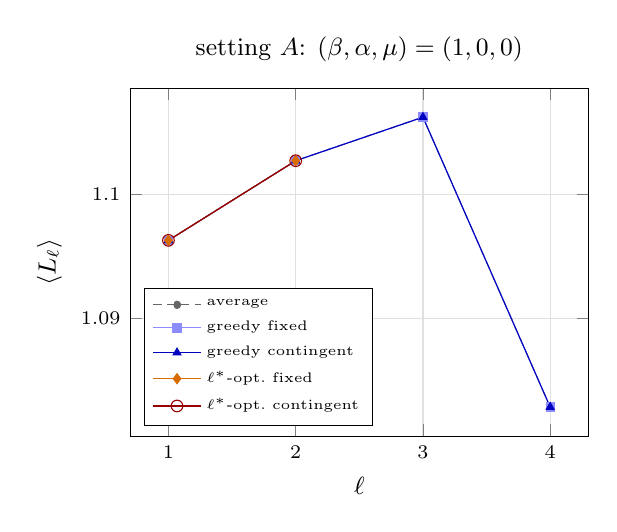
\begin{tikzpicture}
\begin{axis}[width=7.4cm, height=6cm,
  title={setting $A$: $(\beta,\alpha,\mu)=(1,0,0)$},
  title style={font=\small},
  xlabel={$\ell$}, ylabel={$\langle L_\ell \rangle$},
  xtick={1,2,3,4}, grid=major, grid style={black!12},
  tick label style={font=\scriptsize},
  label style={font=\small},
  legend style={font=\tiny, at={(0.03,0.03)}, anchor=south west},
  legend cell align=left]
\addplot[black!60, densely dashed, mark=*, mark size=1.3]
  coordinates {(1,1.0963)(2,1.1027)(3,1.1062)(4,1.0829)};
\addplot[blue!45, mark=square*, mark size=1.5]
  coordinates {(1,1.0963)(2,1.1027)(3,1.1062)(4,1.0829)};
\addplot[blue!75!black, mark=triangle*, mark size=1.6]
  coordinates {(1,1.0963)(2,1.1027)(3,1.1062)(4,1.0829)};
\addplot[orange!85!black, mark=diamond*, mark size=1.8]
  coordinates {(1,1.0963)(2,1.1027)};
\addplot[red!60!black, mark=o, mark size=2.1]
  coordinates {(1,1.0963)(2,1.1027)};
\legend{average, greedy fixed, greedy contingent,
  $\ell^*$-opt.\ fixed, $\ell^*$-opt.\ contingent}
\end{axis}
\end{tikzpicture}\hfill
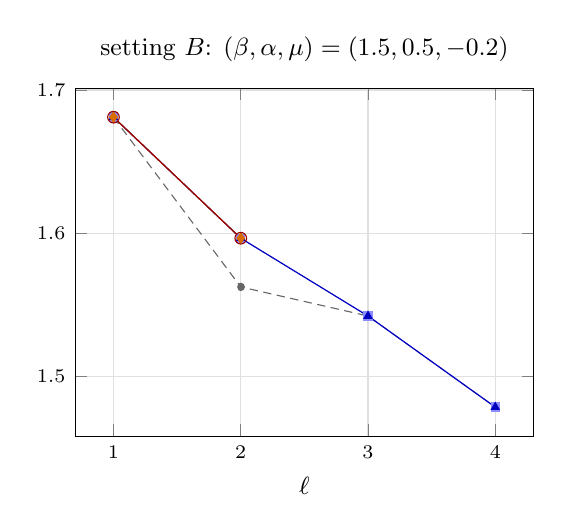
\begin{tikzpicture}
\begin{axis}[width=7.4cm, height=6cm,
  title={setting $B$: $(\beta,\alpha,\mu)=(1.5,0.5,-0.2)$},
  title style={font=\small},
  xlabel={$\ell$}, xtick={1,2,3,4}, grid=major,
  grid style={black!12},
  tick label style={font=\scriptsize}, label style={font=\small}]
\addplot[black!60, densely dashed, mark=*, mark size=1.3]
  coordinates {(1,1.6810)(2,1.5625)(3,1.5422)(4,1.4786)};
\addplot[blue!45, mark=square*, mark size=1.5]
  coordinates {(1,1.6810)(2,1.5965)(3,1.5422)(4,1.4786)};
\addplot[blue!75!black, mark=triangle*, mark size=1.6]
  coordinates {(1,1.6810)(2,1.5965)(3,1.5422)(4,1.4786)};
\addplot[orange!85!black, mark=diamond*, mark size=1.8]
  coordinates {(1,1.6810)(2,1.5965)};
\addplot[red!60!black, mark=o, mark size=2.1]
  coordinates {(1,1.6810)(2,1.5965)};
\end{axis}
\end{tikzpicture}
\caption{Expected leverage under the Gibbs prior at $(2,1)$,
$\ell^* = 2$. Left: under pure Occam all five schedules coincide
exactly. Right: the fields split the schedules at $\ell = 2$.}
\label{fig:gibbs21}
\end{figure}

\begin{figure}[H]
\centering
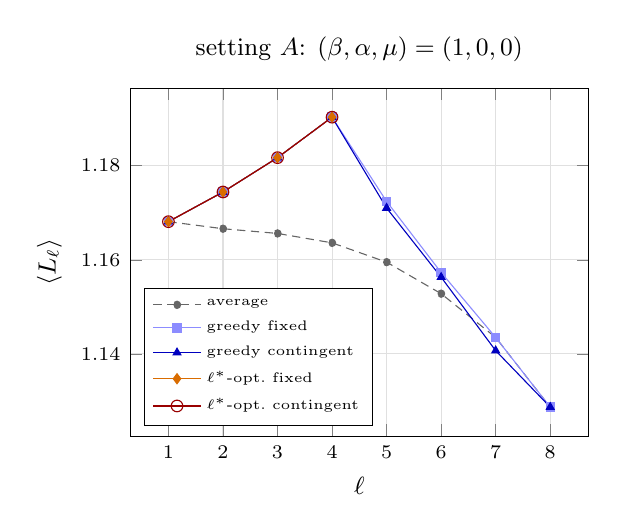
\begin{tikzpicture}
\begin{axis}[width=7.4cm, height=6cm,
  title={setting $A$: $(\beta,\alpha,\mu)=(1,0,0)$},
  title style={font=\small},
  xlabel={$\ell$}, ylabel={$\langle L_\ell \rangle$},
  xtick={1,...,8}, grid=major, grid style={black!12},
  tick label style={font=\scriptsize},
  label style={font=\small},
  legend style={font=\tiny, at={(0.03,0.03)}, anchor=south west},
  legend cell align=left]
\addplot[black!60, densely dashed, mark=*, mark size=1.3]
  coordinates {(1,1.1681)(2,1.1666)(3,1.1656)(4,1.1636)(5,1.1595)
    (6,1.1528)(7,1.1435)(8,1.1287)};
\addplot[blue!45, mark=square*, mark size=1.5]
  coordinates {(1,1.1681)(2,1.1744)(3,1.1817)(4,1.1903)(5,1.1724)
    (6,1.1573)(7,1.1435)(8,1.1287)};
\addplot[blue!75!black, mark=triangle*, mark size=1.6]
  coordinates {(1,1.1681)(2,1.1744)(3,1.1817)(4,1.1903)(5,1.1710)
    (6,1.1563)(7,1.1407)(8,1.1287)};
\addplot[orange!85!black, mark=diamond*, mark size=1.8]
  coordinates {(1,1.1681)(2,1.1744)(3,1.1817)(4,1.1903)};
\addplot[red!60!black, mark=o, mark size=2.1]
  coordinates {(1,1.1681)(2,1.1744)(3,1.1817)(4,1.1903)};
\legend{average, greedy fixed, greedy contingent,
  $\ell^*$-opt.\ fixed, $\ell^*$-opt.\ contingent}
\end{axis}
\end{tikzpicture}\hfill
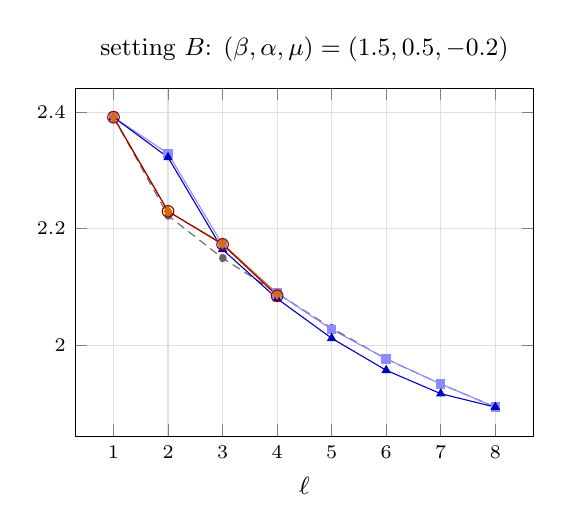
\begin{tikzpicture}
\begin{axis}[width=7.4cm, height=6cm,
  title={setting $B$: $(\beta,\alpha,\mu)=(1.5,0.5,-0.2)$},
  title style={font=\small},
  xlabel={$\ell$}, xtick={1,...,8}, grid=major,
  grid style={black!12},
  tick label style={font=\scriptsize}, label style={font=\small}]
\addplot[black!60, densely dashed, mark=*, mark size=1.3]
  coordinates {(1,2.3915)(2,2.2226)(3,2.1497)(4,2.0894)(5,2.0296)
    (6,1.9764)(7,1.9335)(8,1.8938)};
\addplot[blue!45, mark=square*, mark size=1.5]
  coordinates {(1,2.3915)(2,2.3292)(3,2.1726)(4,2.0895)(5,2.0271)
    (6,1.9767)(7,1.9335)(8,1.8938)};
\addplot[blue!75!black, mark=triangle*, mark size=1.6]
  coordinates {(1,2.3915)(2,2.3225)(3,2.1644)(4,2.0800)(5,2.0120)
    (6,1.9570)(7,1.9168)(8,1.8938)};
\addplot[orange!85!black, mark=diamond*, mark size=1.8]
  coordinates {(1,2.3915)(2,2.2299)(3,2.1744)(4,2.0879)};
\addplot[red!60!black, mark=o, mark size=2.1]
  coordinates {(1,2.3915)(2,2.2299)(3,2.1731)(4,2.0849)};
\end{axis}
\end{tikzpicture}
\caption{Expected leverage under the Gibbs prior at $(3,2)$,
$\ell^* = 4$. Right: at the horizon the $\ell^*$-optimal schedules
know the most and post the \emph{lowest} leverage of the strategic
four -- knowledge and leverage are different objectives.}
\label{fig:gibbs32}
\end{figure}

\begin{figure}[H]
\centering
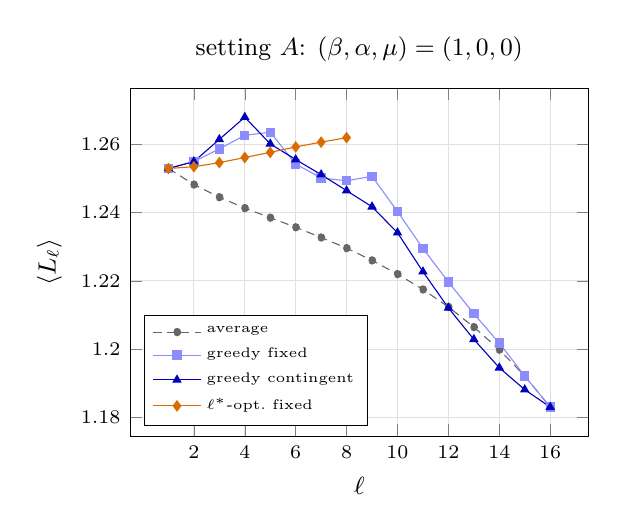
\begin{tikzpicture}
\begin{axis}[width=7.4cm, height=6cm,
  title={setting $A$: $(\beta,\alpha,\mu)=(1,0,0)$},
  title style={font=\small},
  xlabel={$\ell$}, ylabel={$\langle L_\ell \rangle$},
  xtick={2,4,6,8,10,12,14,16}, grid=major, grid style={black!12},
  tick label style={font=\scriptsize},
  label style={font=\small},
  legend style={font=\tiny, at={(0.03,0.03)}, anchor=south west},
  legend cell align=left]
\addplot[black!60, densely dashed, mark=*, mark size=1.3]
  coordinates {(1,1.2529)(2,1.2482)(3,1.2445)(4,1.2413)(5,1.2385)
    (6,1.2357)(7,1.2327)(8,1.2296)(9,1.2260)(10,1.2220)(11,1.2175)
    (12,1.2124)(13,1.2065)(14,1.1999)(15,1.1922)(16,1.1831)};
\addplot[blue!45, mark=square*, mark size=1.5]
  coordinates {(1,1.2529)(2,1.2549)(3,1.2586)(4,1.2626)(5,1.2635)
    (6,1.2542)(7,1.2501)(8,1.2493)(9,1.2506)(10,1.2403)(11,1.2295)
    (12,1.2197)(13,1.2104)(14,1.2018)(15,1.1922)(16,1.1831)};
\addplot[blue!75!black, mark=triangle*, mark size=1.6]
  coordinates {(1,1.2529)(2,1.2549)(3,1.2614)(4,1.2679)(5,1.2601)
    (6,1.2555)(7,1.2511)(8,1.2464)(9,1.2417)(10,1.2341)(11,1.2227)
    (12,1.2121)(13,1.2029)(14,1.1946)(15,1.1882)(16,1.1831)};
\addplot[orange!85!black, mark=diamond*, mark size=1.8]
  coordinates {(1,1.2529)(2,1.2534)(3,1.2546)(4,1.2561)(5,1.2576)
    (6,1.2592)(7,1.2606)(8,1.2619)};
\legend{average, greedy fixed, greedy contingent,
  $\ell^*$-opt.\ fixed}
\end{axis}
\end{tikzpicture}\hfill
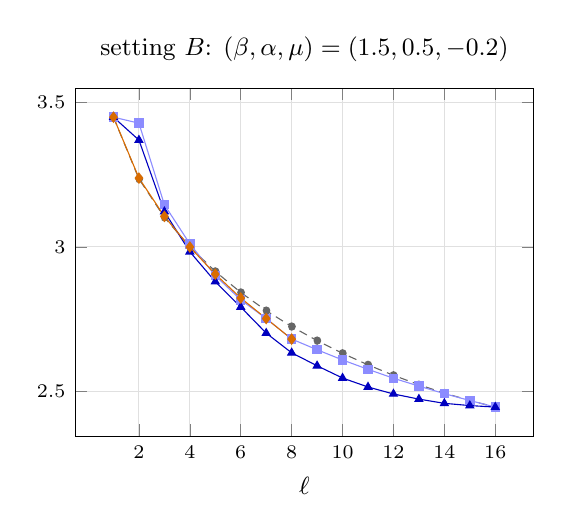
\begin{tikzpicture}
\begin{axis}[width=7.4cm, height=6cm,
  title={setting $B$: $(\beta,\alpha,\mu)=(1.5,0.5,-0.2)$},
  title style={font=\small},
  xlabel={$\ell$}, xtick={2,4,6,8,10,12,14,16}, grid=major,
  grid style={black!12},
  tick label style={font=\scriptsize}, label style={font=\small}]
\addplot[black!60, densely dashed, mark=*, mark size=1.3]
  coordinates {(1,3.4484)(2,3.2350)(3,3.1022)(4,3.0001)(5,2.9151)
    (6,2.8424)(7,2.7796)(8,2.7246)(9,2.6759)(10,2.6320)(11,2.5921)
    (12,2.5560)(13,2.5235)(14,2.4945)(15,2.4689)(16,2.4461)};
\addplot[blue!45, mark=square*, mark size=1.5]
  coordinates {(1,3.4484)(2,3.4276)(3,3.1457)(4,3.0104)(5,2.9005)
    (6,2.8169)(7,2.7522)(8,2.6813)(9,2.6444)(10,2.6090)(11,2.5767)
    (12,2.5459)(13,2.5187)(14,2.4926)(15,2.4689)(16,2.4461)};
\addplot[blue!75!black, mark=triangle*, mark size=1.6]
  coordinates {(1,3.4484)(2,3.3692)(3,3.1218)(4,2.9832)(5,2.8799)
    (6,2.7919)(7,2.7019)(8,2.6338)(9,2.5889)(10,2.5466)(11,2.5156)
    (12,2.4915)(13,2.4737)(14,2.4591)(15,2.4514)(16,2.4461)};
\addplot[orange!85!black, mark=diamond*, mark size=1.8]
  coordinates {(1,3.4484)(2,3.2378)(3,3.1055)(4,2.9995)(5,2.9057)
    (6,2.8232)(7,2.7522)(8,2.6813)};
\end{axis}
\end{tikzpicture}
\caption{Expected leverage under the Gibbs prior at $(4,1)$; only
the contingent optimum is omitted. Under both settings the best
fixed eight questions form a parity class of the input hypercube.
The setting moves the curves by a factor of two and more; the
schedule, by a few percent.}
\label{fig:gibbs41}
\end{figure}

Three observations, one per system size.

At $(2,1)$, under pure Occam, the strategy grid collapses
\emph{exactly}: all six question pairs share a single joint entropy
($1.9679$ bits), so every subset of every size is equivalent and
every schedule is the uniform order. A complexity-only energy at
this size creates correlation without preference. Setting $B$ breaks
the degeneracy -- the footprint and bias fields split the pair
orbits, and the strategic schedules lift above the average at
$\ell = 2$ ($1.5965$ against $1.5625$), greedy attaining the
optimum. The scale jumps too: the colder ensemble stores
$C_0 = 1.074$ bits against setting $A$'s $0.306$.

At $(3,2)$, setting $A$ rewards greed completely: the greedy fixed
set is already the optimal set, and it is the four even-weight
inputs $\{000, 011, 101, 110\}$ -- a maximally spread design, the
questions pairwise at Hamming distance two. Setting $B$ stages the
sharpest lesson of the section. The optimal set
$\{001, 010, 100, 111\}$ differs from greedy's
$\{000, 010, 100, 111\}$ by one question and knows $0.66$ bits more
at the horizon (expected remaining $1.26$ against $1.92$ bits) at an
extra price of $0.32$ received bits -- and its leverage is
\emph{lower}: $2.088$ against greedy's $2.090$. The $\ell$-optimal
schedule maximizes knowledge, not leverage, and a ratio is perfectly
happy with cheaper ignorance. Leverage measures how intelligently a
learner spends, not how much they end up knowing.

At $(4,1)$ the fixed optimum recovers the spread design at scale:
under \emph{both} settings the best eight questions are a parity
class of the input hypercube -- the even-weight inputs, pairwise
Hamming distance two apart (input negation maps the class to its odd
twin, an exactly equivalent design). Under setting $B$ greedy-fixed
lands on that odd twin, and the two curves merge at $\ell = 7, 8$;
under pure Occam greedy's eight questions are \emph{not} a parity
class, and greedy both knows less at the horizon and posts the lower
leverage ($1.249$ against the optimum's $1.262$ -- note the optimal
curve is the only one that \emph{rises} all the way to its horizon).
Setting $B$ pushes the ratio-versus-knowledge caution to its
extreme: at $\ell = 8$ even the strategyless average out-levers the
optimum ($2.725$ against $2.681$) while knowing half as much
(remaining $0.64$ against $0.31$ bits) -- the typical random set is
full of questions the cold prior half-knows already, so it pays
$1.27$ received bits where the maximally informative parity class
pays $1.41$.
Beyond the schedules, the two settings differ far more than the
schedules within either: setting $A$'s curves sit within one percent
of one another, while setting $B$ -- a cold ensemble in earnest,
$H(p) = 1.68$ bits across $65{,}536$ maps -- runs from $3.45$ down
to $2.45$. In the Gibbs world the dominant lever on leverage is the
ensemble's coldness, not the question schedule.

\section{The thermodynamic limit}\label{sec:tdl}

The exact machinery lives on $2^n$ questions; this chapter sends
$n \to \infty$. Time is measured as the asked fraction
$x = \ell / 2^n$, and the object of study is the limiting curve
$L(x)$: what leverage survives when the question space becomes a
continuum. One toy example first, then the general calculus, then a
family of priors solvable in closed form.

\subsection{A toy example: the spike prior}\label{sec:spike}

The simplest prior with something to teach: all conviction on one
map, an honest hedge on the rest. Fix a special map $\phi_\star$
and a weight $p$, and set
%
\begin{equation}
p_\star = p,
\qquad
p_j = \beta := \frac{1-p}{N-1} \quad (j \neq \star),
\qquad N = 2^{m2^n}.
\label{eq:spikeprior}
\end{equation}
%
What makes the spike worth a section is \emph{self-similarity}: the
form \eqref{eq:spikeprior} is closed under the update rule. Asking
any question leaves one of exactly two states. Either the answer
confirms $\phi_\star$ -- probability
%
\begin{equation}
M_\star(p) = p + \Big(\tfrac{N}{2^m} - 1\Big)\beta
\;=\; 2^{-m} + \big(1 - 2^{-m}\big)\,p + O(1/N),
\label{eq:mstar}
\end{equation}
%
and the posterior is again a spike, on the $N 2^{-m}$ surviving
maps, with the sharper weight $p' = p / M_\star(p)$ -- or it refutes
$\phi_\star$, and the posterior is uniform on the survivors, an
absorbing state: a uniform belief stays uniform forever. Because a
single question reproduces the ansatz one size smaller, the spike
lets us zoom in on the effect of \emph{one} question and iterate.
Writing $q_k$ for the probability that the spike has survived $k$
questions,
%
\begin{equation}
q_{k+1} = q_k\, M_\star(p_k),
\qquad
p_{k+1} = \frac{p_k}{M_\star(p_k)},
\qquad q_0 = 1, \; p_0 = p,
\label{eq:spikeflow}
\end{equation}
%
and the product is conserved, $q_k p_k = p_0$ for all $k$: Werner's
unconditional belief in $\phi_\star$ cannot drift in expectation
(the law of iterated expectations -- eliminated maps carry weight
zero, they do not leave the space). The invariant linearizes the
recursion, and with the large-$N$ transition \eqref{eq:mstar},
%
\begin{equation}
q_k = p_0 + (1 - p_0)\,2^{-mk},
\qquad
p_k = \frac{p_0}{p_0 + (1-p_0)\,2^{-mk}}:
\label{eq:spikeclosed}
\end{equation}
%
in odds, each confirming answer delivers exactly $m$ bits of
evidence, and $q_\infty = p_0$ -- the probability of never being
refuted converges to the probability of being right.

Every one-question quantity is now elementary. The two surprisals
are $s_{\checkmark} = -\log_2 M_\star(p)$ and
$s_{\times} = -\log_2\big(1 - M_\star(p)\big)$; the answer-matrix
entropy before the question is $2^n H_{\mathrm{col}}(p)$ with the
column entropy
%
\begin{equation}
H_{\mathrm{col}}(p)
= -P_\star \log_2 P_\star - \big(2^m - 1\big)\,u' \log_2 u',
\qquad
P_\star = p + \tfrac{1-p}{2^m},
\quad u' = \tfrac{1-p}{2^m},
\label{eq:hcol}
\end{equation}
%
and after it, $(2^n - 1) H_{\mathrm{col}}(p_1)$ on the confirming
branch against $(2^n - 1)\,m$ on the refuting one. Splitting the
expected drop of $H(M)$ into received and deduced, and measuring the
deduced part against the store $C = H(M) - H(p)$, gives the
\emph{extraction ratio} $X_1 = D_1 / C \in [0,1]$: the proportion of
the stored knowledge that one question frees.

\begin{figure}[H]
\centering
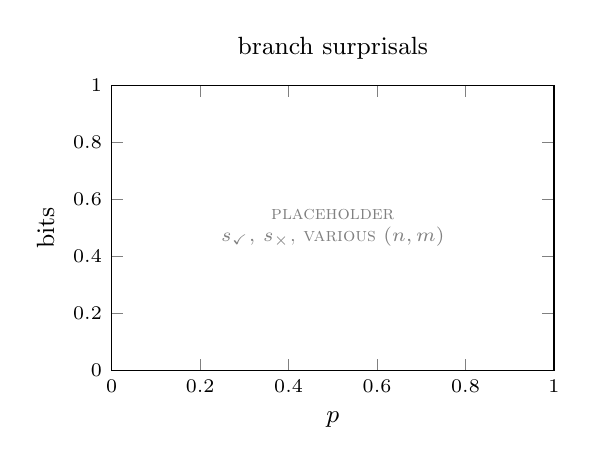
\begin{tikzpicture}
\begin{axis}[width=7.2cm, height=5.2cm,
  title={branch surprisals}, title style={font=\small},
  xlabel={$p$}, ylabel={bits}, xmin=0, xmax=1, ymin=0, ymax=1,
  tick label style={font=\scriptsize}, label style={font=\small}]
\node[gray, font=\scriptsize, align=center, text width=4cm] at (rel axis cs:0.5,0.5)
  {\scshape placeholder \\ $s_{\checkmark},\,s_{\times}$, various $(n,m)$};
\end{axis}
\end{tikzpicture}\hfill
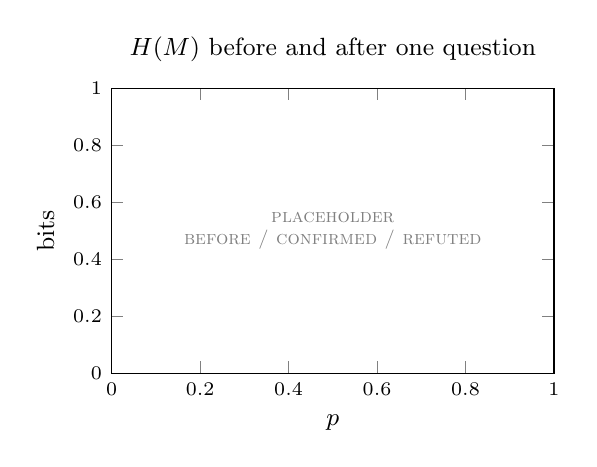
\begin{tikzpicture}
\begin{axis}[width=7.2cm, height=5.2cm,
  title={$H(M)$ before and after one question},
  title style={font=\small},
  xlabel={$p$}, ylabel={bits}, xmin=0, xmax=1, ymin=0, ymax=1,
  tick label style={font=\scriptsize}, label style={font=\small}]
\node[gray, font=\scriptsize, align=center, text width=4cm] at (rel axis cs:0.5,0.5)
  {\scshape placeholder \\ before / confirmed / refuted};
\end{axis}
\end{tikzpicture}

\vspace{2mm}
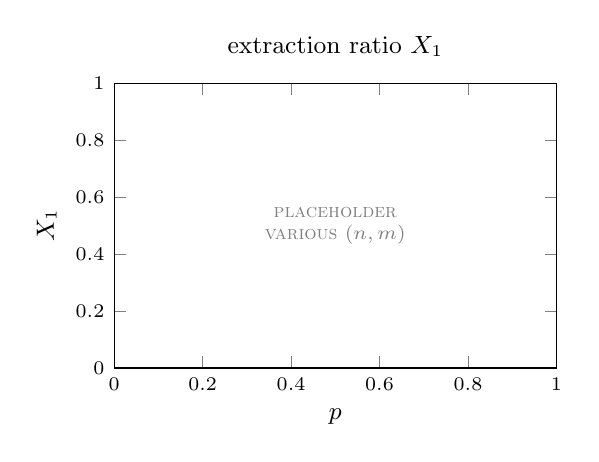
\begin{tikzpicture}
\begin{axis}[width=7.2cm, height=5.2cm,
  title={extraction ratio $X_1$}, title style={font=\small},
  xlabel={$p$}, ylabel={$X_1$}, xmin=0, xmax=1, ymin=0, ymax=1,
  tick label style={font=\scriptsize}, label style={font=\small}]
\node[gray, font=\scriptsize, align=center, text width=4cm] at (rel axis cs:0.5,0.5)
  {\scshape placeholder \\ various $(n,m)$};
\end{axis}
\end{tikzpicture}\hfill
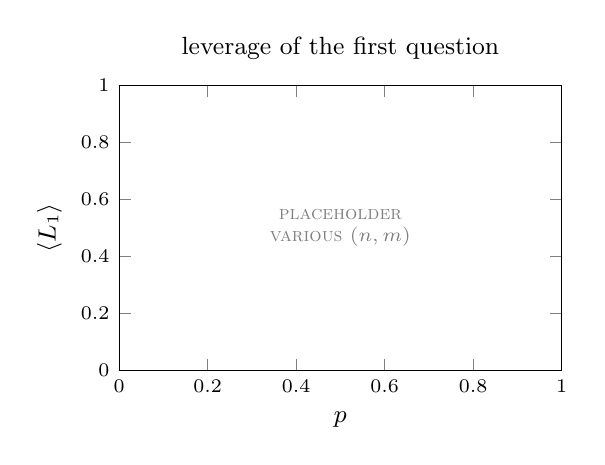
\begin{tikzpicture}
\begin{axis}[width=7.2cm, height=5.2cm,
  title={leverage of the first question},
  title style={font=\small},
  xlabel={$p$}, ylabel={$\langle L_1 \rangle$}, xmin=0, xmax=1,
  ymin=0, ymax=1,
  tick label style={font=\scriptsize}, label style={font=\small}]
\node[gray, font=\scriptsize, align=center, text width=4cm] at (rel axis cs:0.5,0.5)
  {\scshape placeholder \\ various $(n,m)$};
\end{axis}
\end{tikzpicture}
\caption{\emph{Placeholder.} One-question anatomy of the spike prior
as a function of the spike weight $p$, for several $(n, m)$: the two
branch surprisals; the answer-matrix entropy before the question and
on the two branches after it; the extraction ratio; the first
question's leverage.}
\label{fig:spikeone}
\end{figure}

Both ratios have clean sharp limits. As $p \to 1$,
%
\begin{equation}
X_1 \;\longrightarrow\;
\frac{(2^n - 1)\big(1 - 2^{-m}\big)^2}{2^n\big(1 - 2^{-m}\big) - 1}
\;\xrightarrow{\;n \to \infty\;} 1 - 2^{-m},
\qquad
\langle L_1 \rangle \;\longrightarrow\; 2^n - (2^n - 1)\,2^{-m},
\label{eq:spikedelta}
\end{equation}
%
so the first question's leverage is \emph{extensive}, and scaled by
the question count it converges to the same constant:
%
\begin{equation}
\frac{\langle L_1 \rangle}{2^n}
\;\xrightarrow{\;p \to 1,\; n \to \infty\;}\;
1 - 2^{-m}.
\label{eq:cullingratio}
\end{equation}
%
The constant is the \emph{culling ratio}: one answer kills the
fraction $1 - 2^{-m}$ of hypothesis space, and for a near-delta
prior that is also the fraction of every column the answer settles.
The deficit $2^{-m}$ is the probability that total ignorance fakes
the expected answer. The limit is not decoration but necessity: at
$p = 1$ exactly the prior has $H(p) = 0$, the first question
receives nothing and frees nothing, and $L_1$ is the undefined
$0/0$. The spike weight must approach certainty without reaching it,
and the approach is logarithmically slow -- the price of a prior
whose entire store sits one answer deep.

The other order of limits gives the whole trajectory. Fix $p < 1$
and send $n \to \infty$ at asked fraction $x = k/2^n$: the spike
branch sharpens to a delta within $O(1)$ questions -- a vanishing
fraction -- so at every $x > 0$ the two branches have long settled,
and the cumulative leverage converges to a pure hyperbola,
%
\begin{equation}
\big\langle L_{x2^n} \big\rangle
\;\xrightarrow{\;n \to \infty\;}\;
1 + \frac{c(p, m)}{x},
\qquad
c(p, m)
= \frac{H_{\mathrm{col}}(p) - (1-p)\,m}{(1-p)\,m},
\label{eq:spikehyp}
\end{equation}
%
with $H_{\mathrm{col}}$ from \eqref{eq:hcol}. The reading: the
entire store is freed inside a vanishing fraction of the run, and
what the curve records afterwards is that early windfall diluting
into the growing received total. The two orderings do not commute --
$p \to 1$ first gives the extensive plateau
\eqref{eq:cullingratio}, flat in $x$; $n \to \infty$ first gives a
finite hyperbola for every $p < 1$, with $c$ diverging
logarithmically as $p \to 1$.

\begin{figure}[H]
\centering
\begin{tikzpicture}
\begin{axis}[width=9.5cm, height=6cm,
  xlabel={$x = \ell/2^n$}, ylabel={$\langle L \rangle$},
  xmin=0, xmax=1, ymin=0, ymax=1,
  tick label style={font=\scriptsize}, label style={font=\small}]
\node[gray, font=\scriptsize, align=center, text width=6cm] at (rel axis cs:0.5,0.5)
  {\scshape placeholder \\ $1 + c(p,m)/x$ for
   $p \in \{0.001, 0.1, 0.5, 0.9, 0.999\}$};
\end{axis}
\end{tikzpicture}
\caption{\emph{Placeholder.} The limiting spike leverage
\eqref{eq:spikehyp} against the asked fraction, for spike weights
spanning six orders of hedging. All curves share the $1/x$ shape;
the weight only sets the coefficient.}
\label{fig:spikehyp}
\end{figure}

\subsection{Thermodynamic limit calculus}\label{sec:tdlcalc}

The spike's hyperbola is one instance of a general calculus. Recall
the two exact laws of Section~\ref{sec:expectations}: under a random
question order and a truth drawn from the prior, the expected
received after $\ell$ questions is the mean block entropy $G_\ell$,
and the expected remaining answer-matrix entropy is
$(2^n - \ell)(G_{\ell+1} - G_\ell)$. Everything in the limit is
generated by the increments. Define the \emph{profile}
%
\begin{equation}
\gamma(x) := \lim_{n \to \infty}
\big(G_{\lfloor x 2^n \rfloor + 1} - G_{\lfloor x 2^n \rfloor}\big),
\label{eq:profile}
\end{equation}
%
the expected entropy of one more answer given a random $x$-fraction
of the table. By the chain rule this is a conditional entropy, so it
is nonincreasing in $x$ and trapped in $[0, m]$: monotone and
bounded, the best-behaved objects in analysis. Telescoping,
$G_\ell = \sum_{k < \ell} \gamma_n(k)$ is a Riemann sum of the
staircase $t \mapsto \gamma_n(\lfloor t2^n \rfloor)$, and if the
staircase converges pointwise the bounded-convergence theorem passes
it to the integral. Dividing the laws by $2^n$:
%
\begin{equation}
\frac{\mathrm{received}}{2^n} \to g(x) := \int_0^x \gamma(t)\,dt,
\qquad
\frac{\mathrm{remaining}}{2^n} \to (1 - x)\,\gamma(x),
\qquad
L(x) = \frac{\gamma(0) - (1-x)\,\gamma(x)}{g(x)}.
\label{eq:tdlmaster}
\end{equation}
%
Endpoints by first-order expansion: $L(0^+) = 1 -
\gamma'(0)/\gamma(0) \ge 1$ for a differentiable profile, and
$L(1) = \gamma(0)/g(1) = H(M)_0 / H(p)$, the whole-run ratio.

Three assumptions were spent, and each names a way for a prior
family to break the limit. \emph{Extensivity}, at the division:
$H(p^{(n)})$ must scale like $2^n$, or the learning lives on a
sublinear clock and $L$ diverges. \emph{Self-averaging}, at the
pointwise convergence: the staircases of the family
$p^{(n)}$ must settle on a single profile rather than oscillate
with $n$. \emph{Positivity}, $\gamma > 0$ on $[0, 1)$, not needed
for the limit but needed for $L(x)$ to stay regular: a profile that
hits zero at $x^\ast < 1$ compresses an extensive avalanche of
deduction into that instant. Nothing in
\eqref{eq:profile}--\eqref{eq:tdlmaster} chooses a prior: $\gamma$
is computed from any concrete $p^{(n)}$ through its block entropies,
and the rest of this chapter is a gallery of priors whose $\gamma$
comes out in closed form.

\subsection{The coin-flip prior}\label{sec:coins}

The simplest scaling family, worked like a calculus exercise. Take
$R$ coins with biases $\theta_r$ and mixing weights $w_r$: nature
picks coin $r$ with probability $w_r$, then answers every question
independently, each answer bit $1$ with probability $\theta_r$. A
map with $W_j$ ones among its $m2^n$ table bits gets
%
\begin{equation}
p_j = \sum_{r=1}^{R} w_r\,
\theta_r^{W_j} (1 - \theta_r)^{m2^n - W_j}.
\label{eq:coinprior}
\end{equation}
%
At $(2,1)$ with the running example $\theta \in \{0.2, 0.7\}$,
$w = (\tfrac14, \tfrac34)$, the sixteen maps get weights ranging
from $0.0395$ (the half-and-half tables, which neither coin likes)
to $0.1805$ (TRUE): [worked table to be placed here alongside the
derivation steps].

The derivation runs in four steps, each elementary. \emph{One}: at
$\ell = 0$ the predictive is the mean coin, $\gamma(0) =
h(\bar\theta)$ with $\bar\theta = \sum_r w_r \theta_r$. \emph{Two}:
after $\ell$ answers with $k$ ones, the posterior odds between two
coins contain the factor $\ell\big[\tfrac{k}{\ell}\log
\tfrac{\theta_s}{\theta_r} + (1 - \tfrac{k}{\ell})\log
\tfrac{1-\theta_s}{1-\theta_r}\big]$; by the law of large numbers
$k/\ell \to \theta_{\mathrm{true}}$, the bracket converges to a
negative relative entropy, and the wrong coins die exponentially.
\emph{Three}: the predictive converges to the true coin, so for
every fixed $x > 0$ the profile equals the mean coin entropy,
$\gamma(x) = \bar g := \sum_r w_r h(\theta_r)$ -- a step function,
$h(\bar\theta)$ at the single point $x = 0$ and $\bar g$ after.
\emph{Four}: a single point has measure zero, so $g(x) = \bar g x$,
and the master formula collapses to
%
\begin{equation}
L(x) = 1 + \frac{c}{x},
\qquad
c = \frac{h(\bar\theta) - \bar g}{\bar g} \;\ge\; 0
\label{eq:coinhyp}
\end{equation}
%
by Jensen's inequality on the concave $h$. One coin gives $c = 0$,
the product prior, $L \equiv 1$: trivial. And two coins already
exhaust the family: the limit sees the mixture only through the pair
$(h(\bar\theta), \bar g)$, two atoms sweep every admissible pair by
the intermediate value theorem, and de Finetti's theorem closes the
class -- any consistently exchangeable family \emph{is} a coin
mixture. In the thermodynamic limit, two parameters is all the
richness exchangeability has.

\begin{figure}[H]
\centering
\begin{tikzpicture}
\begin{axis}[width=7.4cm, height=5.6cm,
  title={$m = 1$}, title style={font=\small},
  xlabel={$x = \ell/2^n$}, ylabel={$\langle L \rangle$},
  xmin=0, xmax=1, ymin=0, ymax=1,
  tick label style={font=\scriptsize}, label style={font=\small}]
\node[gray, font=\scriptsize, align=center, text width=4.2cm] at (rel axis cs:0.5,0.5)
  {\scshape placeholder \\ $n = 4, 6, 8, 10$ vs $1 + c/x$};
\end{axis}
\end{tikzpicture}\hfill
\begin{tikzpicture}
\begin{axis}[width=7.4cm, height=5.6cm,
  title={$m = 2$}, title style={font=\small},
  xlabel={$x = \ell/2^n$},
  xmin=0, xmax=1, ymin=0, ymax=1,
  tick label style={font=\scriptsize}, label style={font=\small}]
\node[gray, font=\scriptsize, align=center, text width=4.2cm] at (rel axis cs:0.5,0.5)
  {\scshape placeholder \\ $n = 4, 6, 8$ vs $1 + c/x$};
\end{axis}
\end{tikzpicture}
\caption{\emph{Placeholder.} Exact finite-$n$ coin-mixture leverage
converging onto the hyperbola \eqref{eq:coinhyp}, at two answer
widths.}
\label{fig:cointdl}
\end{figure}

The family line is worth drawing: the coin mixture and the spike are
the same mechanism. Both hide \emph{one global secret} -- which
coin, which map -- read off within a vanishing fraction of the run;
both then coast on independent leftovers. That is why both land on
$1 + c/x$: the hyperbola is not a shape the prior chooses but the
signature of front-loaded deduction diluting into the denominator.
Escaping it requires a prior whose secrets cannot all be read at the
start.

\subsection{Non-hyperbolic solvable priors}\label{sec:nonhyp}

What must break is \emph{exchangeability}. A prior invariant under
permuting the questions is, consistently across $n$, a coin mixture,
and Section~\ref{sec:coins} showed those only produce hyperbolas.
Non-hyperbolic limits therefore need priors that treat blocks of
questions differently -- correlations with an address.

The construction: partition the $2^n$ questions into disjoint
\emph{blocks} of size $r$; draw each block's answers independently,
from a distribution symmetric under permuting the block's members.
Independence makes block entropies add; within-block symmetry makes
them depend only on how many of the block's questions have been
asked. Writing $\eta(i)$ for the entropy of one more member given
$i$ already-asked members of its block, the profile follows from a
single limit -- the number of asked partners of a fresh question is
hypergeometric, and sampling without replacement from an enormous
pool becomes binomial:
%
\begin{equation}
\gamma(x)
= \sum_{i=0}^{r-1} b_i(x)\,\eta(i),
\qquad
b_i(x) := \binom{r-1}{i} x^i (1-x)^{r-1-i}.
\label{eq:blockprofile}
\end{equation}
%
The $b_i$ are the \emph{Bernstein basis polynomials}: degree
$r - 1$, positive on $(0,1)$, summing to one, the $i$-th peaked at
$x = i/(r-1)$. At degree three, for instance,
%
\begin{equation}
b_0 = (1-x)^3,\quad
b_1 = 3x(1-x)^2,\quad
b_2 = 3x^2(1-x),\quad
b_3 = x^3.
\label{eq:bernstein3}
\end{equation}

\begin{figure}[H]
\centering
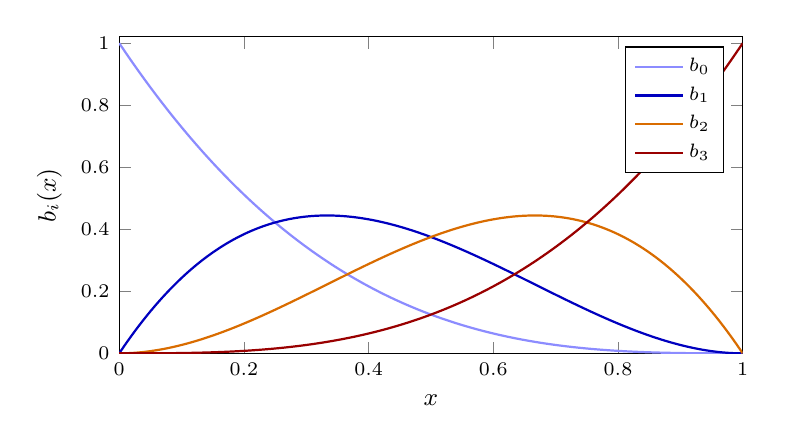
\begin{tikzpicture}
\begin{axis}[width=9.5cm, height=5.6cm,
  xlabel={$x$}, ylabel={$b_i(x)$},
  xmin=0, xmax=1, ymin=0, ymax=1.02,
  domain=0:1, samples=100, smooth,
  tick label style={font=\scriptsize}, label style={font=\small},
  legend style={font=\scriptsize}, legend pos=north east,
  legend cell align=left]
\addplot[blue!45, thick] {(1-x)^3};
\addplot[blue!75!black, thick] {3*x*(1-x)^2};
\addplot[orange!85!black, thick] {3*x^2*(1-x)};
\addplot[red!60!black, thick] {x^3};
\legend{$b_0$, $b_1$, $b_2$, $b_3$}
\end{axis}
\end{tikzpicture}
\caption{The degree-three Bernstein basis \eqref{eq:bernstein3}:
bump functions scanning left to right, each peaked at $i/3$. A block
profile is a positive combination of such bumps, weighted by the
microscopic conditional entropies $\eta(i)$.}
\label{fig:bernstein}
\end{figure}

Equation \eqref{eq:blockprofile} is the whole theory of block
priors: the profile is a Bernstein polynomial whose coefficients are
the block's microscopic conditional entropies, necessarily
nonincreasing in $i$. The shape of $L$ is then a question about
\emph{where the coefficients drop}. Coefficients falling at $i = 0$
front-load the deduction (hyperbola-like decay); a drop at the last
index back-loads it and $L(x)$ \emph{rises}; a drop at an interior
index concentrates the windfall mid-run, and with fresh entropy
after it the leverage becomes non-monotonic -- a genuine interior
peak, impossible for any exchangeable prior.

\subsection{An exotic zoo of solvable priors}\label{sec:zoo}

Five members, each solvable because its $\eta(i)$ is explicit. For
each: the block rule, the profile, the shape.

\emph{Cliques.} All $r$ members share one value, drawn from an
arbitrary block-specific distribution $\nu$: $\eta = (H(\nu), 0,
\ldots, 0)$, so $\gamma(x) = \langle H(\nu)\rangle (1-x)^{r-1}$ and
the scale cancels between destroyed and received:
$L \equiv r$, exactly flat -- every question is either the first
touch of its block (one value received, $r$ columns collapse) or a
free repeat.

\emph{Parity blocks.} Uniform on the strings of fixed parity
$\beta$: any partial view is uniform, so
$\eta = (1, \ldots, 1, 0)$, $\gamma(x) = 1 - x^{r-1}$, and $L$
rises monotonically from $1$ to $r/(r-1)$: the windfall fires only
at a block's last member, deduction back-loaded.

\emph{Tilted parity.} Draw the block's bits i.i.d.\
$\mathrm{Bernoulli}(\theta)$ conditioned on the parity: the general
form, with $\varepsilon := 1 - 2\theta$ as the new parameter. The
conditionals stay closed-form; $\eta(i) = h(\theta) +
O(\varepsilon^{\,r-i})$ far from the cliff and $\eta(r-1) = 0$
exactly: the uniform case is $\varepsilon = 0$, and the tilt lets
partial views leak $O(\varepsilon^{\,r-i})$ bits early, softening
the onset without touching the final deduction.

\emph{MDS blocks.} The block carries a uniformly random codeword of
a code where any $k$ symbols determine all $r$ and any $j \le k$
reveal nothing (Reed--Solomon over $2^m$-ary answers): $\eta = m$
up to $i = k-1$, then $0$, so $\gamma(x)/m = \Pr[\mathrm{Bin}(r{-}1,
x) \le k - 1]$: a movable threshold at $x \approx k/r$. Diluted
with fresh questions the curve climbs to an interior peak and
relaxes -- the non-monotonic shape promised above.

\emph{The cocktail.} A quarter coins, half MDS, a quarter fresh, on
disjoint blocks: profiles average, and the curve inherits all three
mechanisms in sequence -- a hyperbolic dive, a dip, a resurgent
peak, a final decay.

None of the hard members has full support, and all can be given it
without disturbing the limit. The recipe is \emph{local} noise: flip
bits with probability $\delta$ inside a block, or lapse each block
to an i.i.d.\ one with probability $\delta$ -- never a latent shared
across blocks. Locality preserves independence and within-block
symmetry, so the machinery applies verbatim and the noise acts
term by term on the coefficients: the clique's $\eta(i \ge 1)$
lifts from $0$ to the $O(h(2\delta))$ scale; the parity cliff
$\eta(r-1)$ lifts to $h\big(\tfrac{1 - (1-2\delta)^r}{2}\big)$; the
MDS tail lifts to $\approx \delta m$. At fixed $\delta$ the limit
exists and is a continuous deformation of the hard one -- the limit
depends on the noise only through the finitely many $\eta(i)$ --
and under any vanishing schedule $\delta_n \to 0$ the prior has
full support at every finite $n$ while the limit is \emph{exactly}
the hard curve. What must be avoided is global softening: a shared
latent with extensive entropy floods the received channel and can
erase the store outright.

Nothing here is finely tuned. An \emph{arbitrary} mixture of block
types -- fractions $w_t$ of questions in blocks of size $r_t$ with
any within-block-symmetric distributions -- is solvable by the same
one formula,
%
\begin{equation}
\gamma(x) = \sum_{t} w_t \sum_{i=0}^{r_t - 1}
b^{(r_t - 1)}_i(x)\,\eta_t(i),
\label{eq:zoomix}
\end{equation}
%
symbolically, before any constituent is specified: the $\eta_t(i)$
are the only inputs, and mixing blocks mixes their profiles
linearly (the leverage, a ratio, then mixes as a mediant). The
solvability is a property of the block structure, not of a lucky
choice of members.

\begin{figure}[H]
\centering
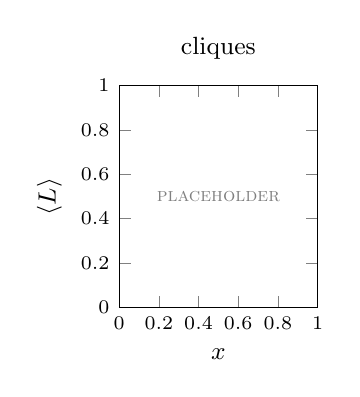
\begin{tikzpicture}
\begin{axis}[width=4.1cm, height=4.4cm,
  title={cliques}, title style={font=\small},
  xlabel={$x$}, ylabel={$\langle L \rangle$},
  xmin=0, xmax=1, ymin=0, ymax=1,
  tick label style={font=\scriptsize}, label style={font=\small}]
\node[gray, font=\scriptsize] at (rel axis cs:0.5,0.5)
  {\scshape placeholder};
\end{axis}
\end{tikzpicture}\hfill
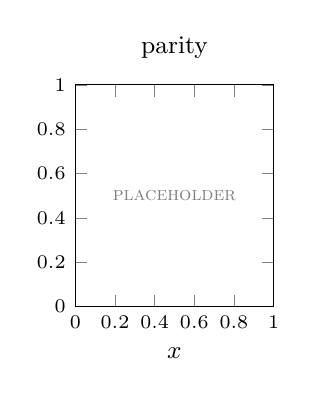
\begin{tikzpicture}
\begin{axis}[width=4.1cm, height=4.4cm,
  title={parity}, title style={font=\small},
  xlabel={$x$}, xmin=0, xmax=1, ymin=0, ymax=1,
  tick label style={font=\scriptsize}, label style={font=\small}]
\node[gray, font=\scriptsize] at (rel axis cs:0.5,0.5)
  {\scshape placeholder};
\end{axis}
\end{tikzpicture}\hfill
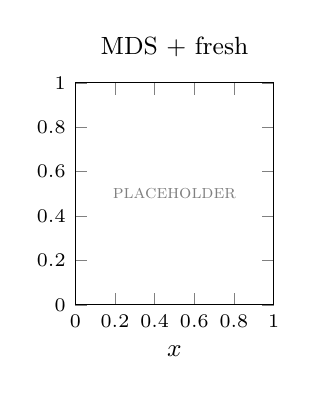
\begin{tikzpicture}
\begin{axis}[width=4.1cm, height=4.4cm,
  title={MDS + fresh}, title style={font=\small},
  xlabel={$x$}, xmin=0, xmax=1, ymin=0, ymax=1,
  tick label style={font=\scriptsize}, label style={font=\small}]
\node[gray, font=\scriptsize] at (rel axis cs:0.5,0.5)
  {\scshape placeholder};
\end{axis}
\end{tikzpicture}\hfill
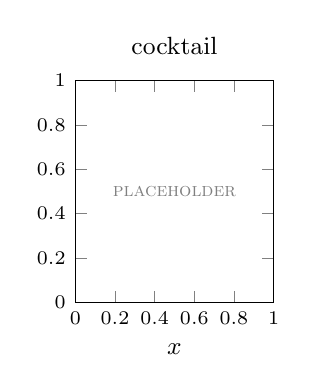
\begin{tikzpicture}
\begin{axis}[width=4.1cm, height=4.4cm,
  title={cocktail}, title style={font=\small},
  xlabel={$x$}, xmin=0, xmax=1, ymin=0, ymax=1,
  tick label style={font=\scriptsize}, label style={font=\small}]
\node[gray, font=\scriptsize] at (rel axis cs:0.5,0.5)
  {\scshape placeholder};
\end{axis}
\end{tikzpicture}
\caption{\emph{Placeholder.} The zoo side by side: flat, rising,
peaked, and the cocktail's dive--dip--peak--decay, each with exact
finite-$n$ curves converging on its limit.}
\label{fig:zoo}
\end{figure}

\begin{center}
\begin{tabular}{lllll}
\toprule
member & block rule & $\eta(i)$ & $\gamma(x)$ & $L(x)$ \\
\midrule
cliques & one shared value $\nu$ &
  $H(\nu), 0, \ldots$ &
  $\langle H(\nu)\rangle(1{-}x)^{r-1}$ &
  $\equiv r$, flat \\
parity & uniform, $\oplus = \beta$ &
  $1, \ldots, 1, 0$ &
  $1 - x^{r-1}$ &
  rises to $\tfrac{r}{r-1}$ \\
tilted parity & i.i.d.\ $\theta$ given $\oplus = \beta$ &
  plateau, cliff &
  closed form in $\varepsilon$ &
  rises, soft onset \\
MDS $+$ fresh & uniform codebook &
  $m, \ldots, m, 0, \ldots$ &
  $w\bar F + (1{-}w)$ &
  peak near $k/r$ \\
cocktail & coins, code, fresh &
  mixture &
  mixture &
  dive, dip, peak \\
\bottomrule
\end{tabular}
\end{center}

The zoo earns a closing remark. Each member's limiting curve is the
visible fingerprint of an invisible structure: hyperbolas betray one
global secret, flat lines betray duplication, rising curves betray
constraints that bind only when complete, peaks betray thresholds.
The inference runs backwards as well as forwards. A well pre-trained
model traces an empirical $L(x)$ as it learns, and the shape of that
learning curve -- falling, flat, rising, peaked -- is evidence about
which class of prior the real world's regularities are drawn from.
Measuring how a learner's leverage evolves may be the most practical
window we have onto the distribution type of the world itself.

\end{document}
